%% NOTE: the submission version is main_oup.tex (OUP template); keep both in sync or edit only main_oup.tex.
\documentclass[12pt,a4paper]{article}
\usepackage[utf8]{inputenc}
\usepackage{amsmath}
\usepackage{placeins}
\usepackage{url}
\usepackage{svg}
\usepackage{natbib}
\usepackage{titlesec}
\usepackage{color,xcolor,setspace,geometry}
\setcitestyle{authoryear,open={(},close={)}}
\usepackage{cite}
\usepackage{soul}
\usepackage{mathtools}
\usepackage{bbm}
\usepackage{dsfont}
\soulregister\citep7
\soulregister\cite7
\soulregister\citet7
\soulregister\citealp7
\soulregister\ref7
\usepackage{amsfonts}
\usepackage{tikz}
\usetikzlibrary{shapes}
\usetikzlibrary{plotmarks}
\usetikzlibrary{tikzmark,matrix,calc}
\usetikzlibrary{arrows.meta,calc,decorations.markings,math,arrows.meta}
\usepackage{amssymb}
\usepackage{multirow}
\usepackage{hyperref}
\usepackage{todonotes}
\usepackage{graphicx}
\usepackage{array}
\usepackage{bm}
\usepackage{arydshln}
\usepackage[final]{changes}
\geometry{verbose,letterpaper,tmargin=3cm,bmargin=3cm,lmargin=3.2cm,rmargin=3.2cm}
\titleformat*{\section}{\large\bfseries}
\titleformat*{\subsection}{\bfseries}

\providecommand{\keywords}[1]
{
  \small	
  \textbf{\textit{Keywords---}} #1
}

%\newcommand{\highlight}[1]{%
%  \colorbox{yellow}{$\displaystyle#1$}}


\newcommand{\blue}[1]{\textcolor{blue}{#1}}
  
\usepackage{natbib}
\usepackage{datatool}
\usepackage{etoolbox}

\newcommand{\highlightmath}[1]{\colorbox{yellow}{$\displaystyle#1$}}

\DTLnewdb{bibnotes}

\def\bibnote#1#2{
  \DTLnewrow{bibnotes}
  \DTLnewdbentry{bibnotes}{mylabel}{#1}
  \DTLnewdbentry{bibnotes}{mynote}{#2}
}

\makeatletter
\patchcmd{\@lbibitem}
  {\item[\hfil\NAT@anchor{#2}{\NAT@num}]}
  {
    \item[\hfil\NAT@anchor{#2}{\NAT@num}]
    \DTLforeach[\DTLiseq{\mylabel}{#2}]{bibnotes}{\mylabel=mylabel,\mynote=mynote}{\text{\mynote}}
  }{}{\message{^^JPatching failed^^J}}

\newcommand{\subsubsubsectionline}[1]{\vspace{0.5em}\noindent\textit{#1}\par\vspace{0.25em}}

\newcommand{\robert}[1]{\textcolor{green!50!black}{RB: #1}}
\newcommand{\rmr}[1]{\textcolor{black!40}{rm(RB): #1}}

\newcommand{\indep}{\protect{\perp\!\!\!\perp}}
\newcommand{\given}{\mid}
\newcommand{\RR}{\mathbb{R}}
\DeclareMathOperator*{\argmax}{arg\,max}

\makeatother
% Alternative text for figures, as required by the journal (shown under each
% caption in the submitted manuscript, not in the typeset article).
% Switch: \showalttexttrue for the submission, \showalttextfalse to hide them.
\newif\ifshowalttext
\showalttextfalse
\newcommand{\alttext}[1]{\ifshowalttext\par\smallskip{\footnotesize\noindent Alt text: #1}\fi}
\begin{document}
\begin{spacing}{1.35}

%\title{Capturing dependencies nonparametrically in multivariate hidden Markov models}
\title{Integrating Unsupervised and Supervised Learning for the Prediction and Interpretation of Defensive Schemes in American Football}
\author{Rouven Michels\thanks{Corresponding author: Rouven Michels, Department of Statistics, TU Dortmund University, 44221 Dortmund, Germany; rouven.michels@tu-dortmund.de} \thanks{TU Dortmund University, Germany}, Robert Bajons\thanks{WU Vienna, Austria}, Jan-Ole Fischer\thanks{Bielefeld University, Germany}}
\date{Running head: Defensive coverage schemes from tracking data}

\maketitle

\begin{abstract} 
\noindent
Anticipating defensive coverage schemes is a crucial yet challenging task for offenses in American football, as defenders’ assignments are intentionally disguised before the snap. We develop a statistical framework that integrates unsupervised and supervised learning using player tracking data. A non-homogeneous hidden Markov model with random effects for positions, teams and plays infers latent guarding assignments between defensive and offensive players during pre-snap motion. The model offers interpretable insights into defensive behaviour, quantifying the defenders' reaction time, the persistence of their guarding assignments and how it differs between positions, teams and plays. Features derived from the posterior state probabilities complement pre-motion and naive post-motion features in elastic net logistic regression and gradient-boosted decision trees that forecast whether the defense plays man or zone coverage. The latent-state features are significantly associated with the coverage scheme beyond simple motion summaries; given the limited number of plays, however, this information translates only into small predictive gains, which are consistent for the elastic net. As the estimated dynamics are stable and the fitted model can be applied to new plays at negligible cost, the approach scales to larger data sets, in which this information may be exploited more fully.
\end{abstract}
\keywords{American football, forecasting, hidden Markov model, random effects, XGBoost}

\section{Introduction}

In American football, one of the most critical strategic questions an offense faces is identifying the defensive coverage scheme before the snap. Whether the defense is aligned in man- or zone coverage dictates the effectiveness of route combinations, blocking assignments, and ultimately the success of an offensive play. A central tool offenses employ to gain information about the defensive scheme is pre-snap motion. By moving receivers, tight ends, or running backs, coordinators seek to trigger visible reactions from defenders that provide cues about their coverage responsibilities. If a cornerback follows a motioning receiver across the entire field, this may indicate a man-to-man coverage scheme; if defenders pass on offensive players and shift in the direction of the motion, zone coverage becomes more likely. Thus, pre-snap motion serves as a diagnostic tool to gain information on the defensive scheme.

Historically, the interpretation of pre-snap movements has been almost entirely visual. Coaches and analysts rely on film study to infer how defenses react to offensive formations and motions. While this process has proven effective in practice, it remains subjective.
The increasing availability of player tracking data offers a way to overcome these limitations. These data include spatial information on player movements, thereby fundamentally changing how defensive coverages --- and football situations more broadly --- can be evaluated. 
Over the past decade, the integration of play-by-play and tracking data has reshaped multiple domains of football analytics, for example, fourth-down decision-making \citep{sandholtz2024learning, brill2025analytics}, the in-game valuation of plays \citep{yurko}, the understanding of pass rushes \citep{nguyen}, and the contribution of tackles \citep{bajons2025pep}. A notable step towards the prediction of coverage schemes was made by \citet{dutta2020unsupervised}, who employed mixture models to infer defensive assignments from player tracking data. While this approach demonstrated the potential of data-driven inference for coverage identification, it did not incorporate information on pre-snap motion. However, this phase may hold valuable latent patterns that can be statistically inferred and leveraged for improved coverage identification.

To fill this gap, we aim to predict the overall coverage scheme through a hybrid statistical framework combining unsupervised and supervised learning using play-by-play and tracking data from the first nine weeks of the 2022 NFL season. Specifically, we classify man- or zone coverage with an elastic net logistic regression and gradient-boosted decision trees based on contextual and spatial features from pre- and post-motion phases. 
To identify coverage patterns based on observed player movements while accounting for persistence in latent guarding assignments, we employ hidden Markov models (HMMs).
HMMs are a versatile statistical framework for modelling time series driven by underlying, unobserved states and have been applied to various fields, including finance \citep{liu2012stock, zhang2019high}, ecology \citep{mcclintock2020uncovering, mews2022multistate}, and medicine \citep{amoros2019continuous, soper2020hidden}.
Moreover, latent-state time-series models have been employed across multiple sports analytics domains to uncover unobserved structures, such as tactics (\citealp{otting2023football, adam2024markov}) or hot hand and momentum effects (\citealp{albert93, michels2023bettors, winkelmann2025momentum}).

In our case, we employ a non-homogeneous HMM to infer latent guarding assignments between defensive and offensive players during the pre-snap motion phase. For this, we model the defenders’ trajectories in each play conditional on the offensive players' positions. Local decoding of each defender’s time series provides probabilistic information on the guarding assignments from each defensive player to each offensive player in each play. 
The results from the HMM are then transferred into suitable and interpretable summary statistics, computed as expectations under the posterior distribution of the latent guarding assignments, and incorporated as features in the supervised learning models.
The fitted HMM is interpretable in its own right: it quantifies the defenders' reaction time, the persistence of their guarding assignments and how this persistence differs between positions, teams and plays. In addition, we assess the value of the HMM-derived features for predicting the coverage scheme in two complementary ways. First, we compare the prediction of man- or zone coverage with regard to several common loss metrics with and without HMM-derived features. While most of the predictive gain stems from naive post-motion features, adding the HMM-derived features yields small but consistent improvements for the elastic net. %By devising a suitable cross-fitting procedure, we are able to reveal that the models incorporating HMM features improve out-of-sample performance compared to models solely relying on naive pre- and post-motion features. 
Second, by leveraging recently established non-parametric conditional independence tests and more specifically the Generalized Covariance Measure (GCM) test \citep{Shah20gcm}, we show that the HMM features are significantly associated with the coverage outcome, even given the pre- and naive post-motion features. Furthermore, using results from \citet{bajons2025rGAX}, the GCM test provides interpretable insights into the influence of the HMM features on the outcome. Together, these results show that the HMM features carry genuine information on the coverage scheme, whose predictive value is, however, limited by the small number of plays available. Finally, we use the XGBoost coverage models to examine team behaviour and motion patterns. More specifically, we analyse which teams are able to exploit motion in order to more effectively determine defensive coverage schemes. 

The paper is organized as follows. Section~\ref{sec:data} describes the data. Section~\ref{sec:methods} presents the methodology, including the unsupervised and supervised modelling components. Section~\ref{sec:results} reports the results. Section~\ref{sec:discussion} concludes with a discussion.

\section{Data}
\label{sec:data}
\begin{figure}[t!]
    \centering
    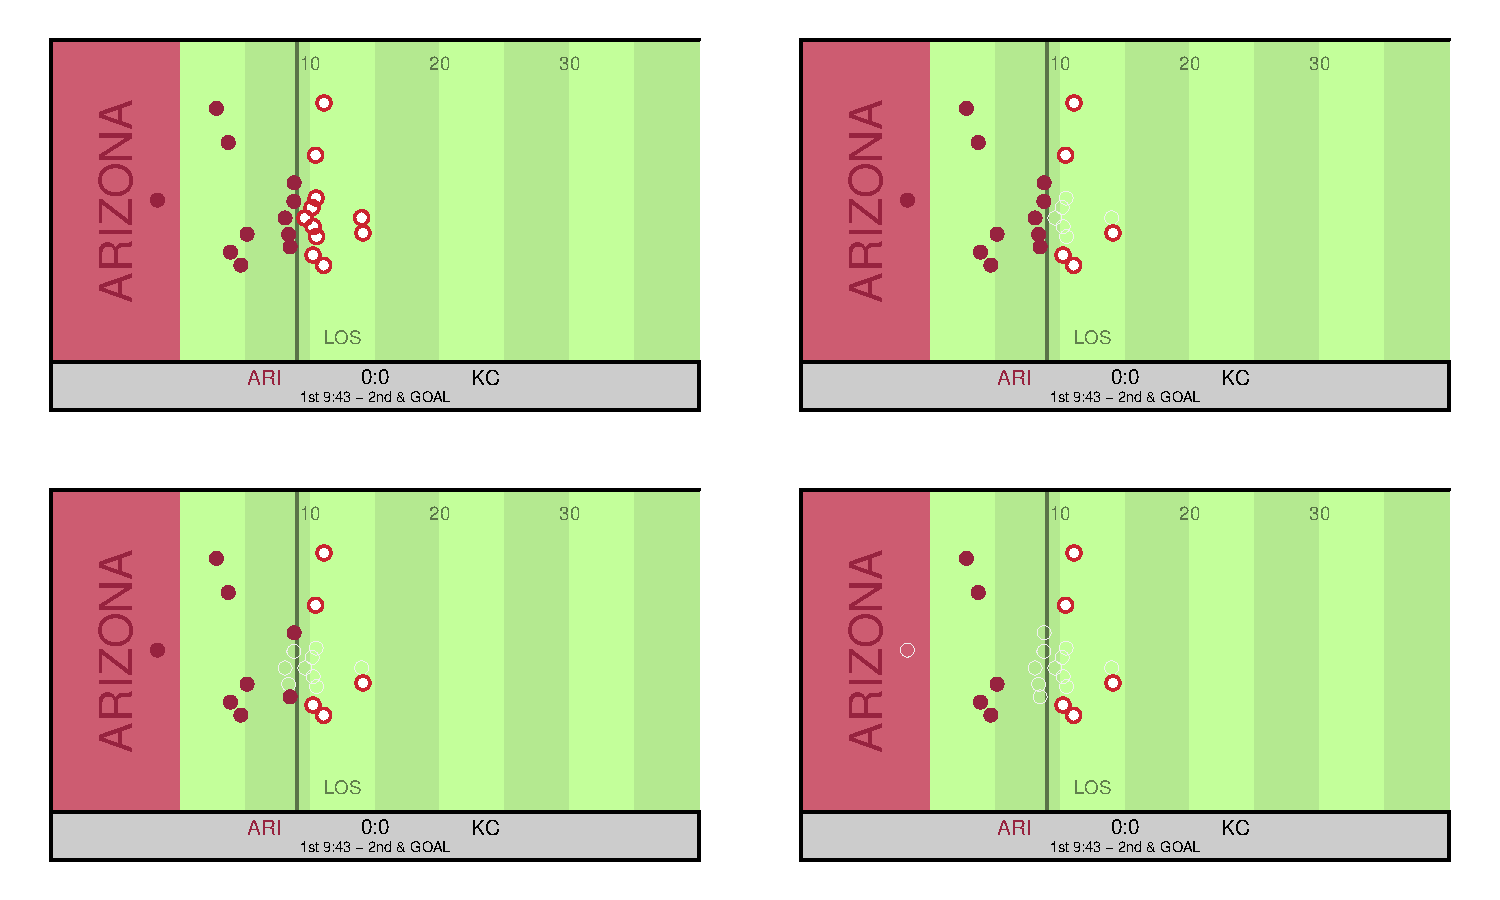
\includegraphics[width=\linewidth]{figures//plots/Data_preprocessing2.pdf}
    \caption{This figure illustrates the step-by-step pre-processing for a game between the Arizona Cardinals and the Kansas City Chiefs. From top left to bottom right, we first display all players, then exclude offensive non-skill players, next omit defensive linemen, and finally remove pass-rushing linebackers and the deepest defenders. Grey circles mark the players excluded during each pre-processing step.}
    \label{fig:prepro}
    \alttext{Four panels showing the players of one play on a football field, with fewer players highlighted in each panel as offensive linemen, quarterback, defensive linemen, pass rushers and the deepest defenders are removed, leaving five offensive and five defensive players.}
\end{figure}

The analysis in this paper is based on data provided as part of the NFL Big Data Bowl (BDB) 2025, specifically tracking data, sampled at 10 Hz, and play-by-play data from the first nine weeks of the 2022 NFL season. While the former provides information on the locations of every player on the field during a play, the latter contains general, contextual information on the respective plays. As we are interested in analysing pre-snap player movements, we concentrate on plays that contain any pre-snap motion from the offense. For each play, the time series starts at the first time the offense is set (event \texttt{line\_set}) and ends at the snap. Moreover, we omit plays from jumbo and wildcat formations as well as plays with more than five offensive linemen or two quarterbacks on the field. Ultimately, we end up with $M = 4344$ offensive plays in total, of which the different defenses played $3252$ in zone and $1092$ in man coverage. 

Our modelling framework is structured into three stages: a pre-motion model, a naive post-motion model, and a post-motion model including HMM features. Thereby, the amount of available information progressively increases. Each subsequent stage builds upon the data used in the previous models.
Starting with the creation of the pre-motion data set, we first extract information from the play-by-play data, specifically the current quarter, down, yards to go, yardline, home and away scores, the remaining seconds in the current half, and, most importantly, whether the defense played man- or zone coverage\footnote{Note that this information is itself provided by the company Pro Football Focus as part of the NFL BDB data.}. In addition, we create different features derived from the tracking data that describe the situation before any player motions. In particular, we first compute the area spanned by the convex hull of all players from both teams, as well as the largest y-distance (i.e., the width of the hull) and the largest x-distance (i.e., the length of the hull) of both convex hulls. 
Subsequently, we concentrate on the offensive players that can potentially move before the snap, i.e., exclude offensive linemen and the quarterback. This yields five offensive skill players (an arbitrary combination of running backs, full backs, tight ends, and wide receivers) for each individual play. 
To enable direct man-to-man assignments later in the HMM framework, we match the number of defensive players with the five offensive players. For that, we omit defensive linemen (nose tackles, defensive tackles, and defensive ends) and those players that are tagged as linebackers but align directly at the line of scrimmage (within two yards of the ball) as pass rushers (players such as Micah Parsons).
Afterwards --- if more than five defenders remain --- we exclude the defenders other than cornerbacks that are aligned deepest, i.e., farthest from the line of scrimmage, typically deep safeties, which leads to $5 \times M = 21{,}720$ time series. Figure~\ref{fig:prepro} exemplifies all these pre-processing steps for a play between the Arizona Cardinals and the Kansas City Chiefs in Week 1, which will serve as a running example throughout this manuscript.
From these remaining ten players, we derive twenty features related to their (standardized) position. A detailed description is provided in Section~3 of the  Supplementary Material.

%Each observation corresponds to a unique frame within a play and includes the (x,y) coordinates of every player on the field, their speed, acceleration, orientation, and team affiliation, as well as contextual information such as down, distance, and game situation.
In a second step, to create the naive post-motion data set, we capture post-motion information purely from tracking data. In particular, we introduce six features: for both the offense and defense, we compute the maximum distance along the x- and y-axes, as well as the total
distance traveled by all players between the start of the motion and the snap. These features are added to those used in the pre-motion model.

Finally, the HMM data set combines all previously derived features with additional variables obtained from suitable summary statistics of the posterior state probabilities. Information on how this dataset was created is provided in Section~\ref{sec:summary}. Throughout this process, no modifications were made to the raw time-series structure of the tracking data so as to preserve its underlying temporal structure (\citealp{michels2024combination}).

\section{Methods}\label{sec:methods}

Our modelling framework is designed in two layers. On the outer level, we employ two supervised learning models to predict the defensive coverage scheme based on contextual and spatial features described in the previous section. However, one of the most informative indicators for the defensive scheme, the assignments of defenders to offensive players, is not directly observable. Thus, we use a hidden Markov model as the inner component of our statistical framework to generate additional latent-state features that serve as inputs for the supervised models.

\subsection{Unsupervised learning}
As the unsupervised learning part, we use a hidden Markov model to infer guarding assignments between offensive and defensive players. HMMs are particularly well-suited for this task since these guarding assignments are not directly observable but must be inferred from the defenders' responses to the offensive players' movements. 
In this section, we describe our formulation and estimation of the HMM and explain how decoded state probabilities are incorporated as features into the supervised models.

\subsubsection{HMM formulation}

An HMM consists of two stochastic processes: an observed process $\{Y_t\}_{t=1}^{T}$ and an unobserved first-order Markov chain $\{ S_t\}_{t=1}^{T}$, with $S_t \in \{1,\ldots,N\}$ where $N$ is the number of states. The connection of both processes arises from the assumption that the observations $y_t$ --- in our case, literally the (vertical) $\mathrm{y}$-coordinates of the individual defenders in each play --- are generated by a state-dependent distribution that, in a basic model, only depends on the currently active state $S_t$. More formally, for each defender's trajectory $\{Y_t\}$, we assume that
\begin{equation}
\label{ind}
f(y_t \mid s_1, \ldots, s_t, y_1, \ldots, y_{t-1},y_{t+1},\ldots,y_{T_m}) = f(y_t \mid S_t = s_t),
\end{equation}
where $s_t \in \{1, \ldots, N\}$ and $t = 1, \ldots, T_m$, with $m = 1, \ldots, M$ specifying the m-th play. Note that, according to this model formulation, we model the guarding assignments of every individual defender. Thus, we assume that the trajectories of individual defenders are statistically independent from those of their teammates. Hence, it is possible that multiple defenders are assigned to one of the $N$ offensive players in a specific play $m$ (which, in reality, does happen), but not vice versa. 
We set $N=5$ due to the predetermined number of five offensive skill players that can potentially be guarded. 

\begin{figure}[t!]
    \centering
    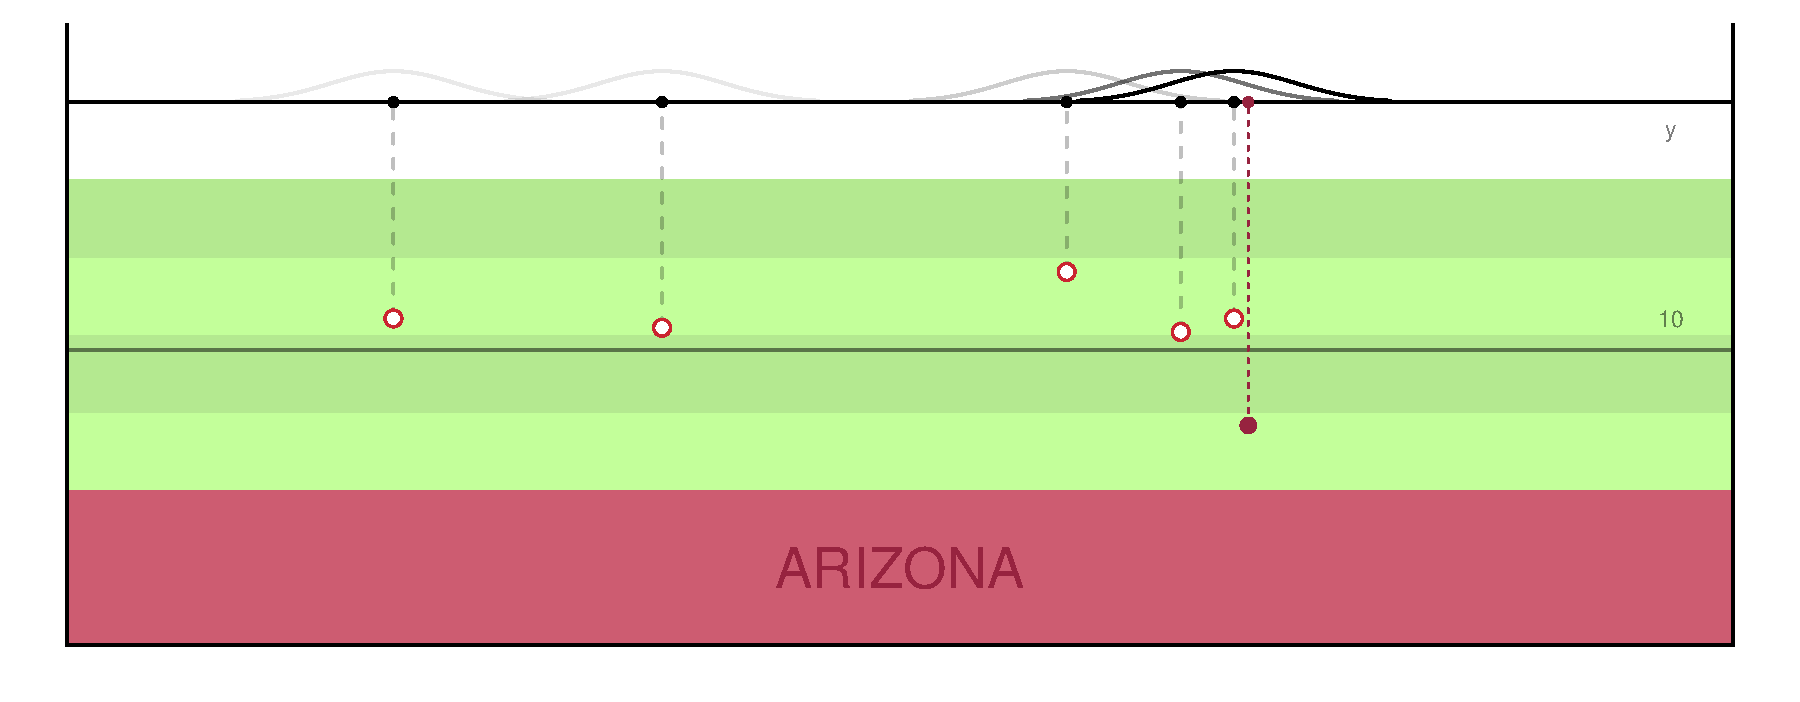
\includegraphics[width=\linewidth]{figures//plots/HMM_expl.pdf}
    \caption{This figure illustrates the HMM modelling approach. Specifically, we project the $(x,y)$-coordinates of the players onto a single $\mathrm{y}$-axis. We assume that the observations $y_t$, i.e., the defensive players' $\mathrm{y}$-coordinate, is generated by one of the five Gaussian state-dependent distributions, whose mean equals the $\mathrm{y}$-coordinate of the five offensive players.}
    \label{fig:HMMexpl}
    \alttext{Players of a play projected onto the lateral axis; five normal densities centred at the lateral positions of the five offensive players illustrate the state-dependent distributions of a defender's position.}
\end{figure}

We operationalize Eq.~\ref{ind}, by assuming that, at each time point $t$, every defender's $\mathrm{y}$-coordinate is a realization from a mixture of Gaussian distributions, where each mixture component represents the location of one offensive player (see \citealp{franks2015} for a similar approach in basketball). 
More formally, a natural candidate for the state-dependent distributions is
\begin{equation}
\label{eqn:state_dep}
  f(y_t \mid S_t = j) \sim \mathcal{N}(\mu_{t,j}, \sigma^2), \quad j = 1, \ldots, 5,  
\end{equation}
where the standard deviation $\sigma$ is estimated and the mean
% $$\mu_{t,j} = y_{\text{off}_{j, t}},$$ 
$$\mu_{t,j} = \mathrm{y}_t(\text{off}_j),$$ 
which denotes the $\mathrm{y}$-coordinate of offensive player $j$ at time $t$. The idea behind this modelling framework is that we expect defenders to mirror the offensive players at the line of scrimmage once teams come out of the huddle (see Figure~\ref{fig:HMMexpl}) and, in the case of tight coverage, also throughout the motion phase. 
A distinctive characteristic of the motion phase is that when offensive players move, defenders react to that movement. Thus, a more realistic model accounts for the time it takes for the defender to react to the offensive players' movement (see \citealp{wu2023evaluation} for a similar idea in soccer). Hence, we extend the basic modelling framework and allow for lagged observations within the mean of the state-dependent distribution, i.e., 
\begin{equation}\label{eq:lag}    
%\mu_{t,j} = \mathrm{y_\text{off}}^{j}_{t-l},
\mu_{t,j} = \mathrm{y}_{t-l}(\text{off}_j),
\end{equation}
with the lag $l$ being a proxy for the average reaction time of defenders. 
Given the 10 Hz temporal resolution of the data, $l$ can be interpreted as the number of tenths of a second it takes a defender to respond to an offensive player’s movement. For instance, $l = 4$ corresponds to an average reaction time of 0.4 seconds.

\subsubsection{Modelling the underlying Markov chain}
\label{sec:MC_dets}

Within our HMM (see Figure~\ref{fig:HMM} for a visualization of the basic structure), the unobserved state process is modelled as a first-order Markov chain. This is described by an initial distribution 
$$\boldsymbol{\delta}^{(1)} = \bigl( \Pr(S_1=1), \ldots, \Pr(S_1=5) \bigr),$$ 
that specifies the probability of every defender to guard the respective offensive players at the beginning of the time series, and a transition probability matrix (t.p.m.) 
$$\boldsymbol{\Gamma} = (\gamma_{ij}),\ \text{with} \  \gamma_{ij} = \Pr(S_t = j \mid S_{t-1} = i), \quad i,j = 1, \ldots, 5$$
The latter specifies the probability of a defender switching from guarding offensive player~$i$ at time~$t-1$ to offensive player~$j$ at time~$t$.
In a simple model, we would estimate a single, homogeneous transition probability matrix (t.p.m.). However, we seek to obtain a more realistic representation of the switching probabilities by allowing them to vary with covariates. 
Clearly, if a defender is currently guarding offensive player~$i$, a switch to guarding another offensive player~$j$ is more likely if those two are close in distance with respect to the $\mathrm{y}$-coordinate. Hence, we incorporate the pairwise distance between offensive players, i.e., $\vert \mathrm{y}_{t-l}(\text{off}_i) - \mathrm{y}_{t-l}(\text{off}_j) \vert$ for $i,j = 1, \ldots, 5$, as a covariate.
Further, we account for systematic heterogeneity across different positions, teams, and plays by including specific random effects in the state-transition probabilities (\citealp{maruotti2009semiparametric}). Thus, for the positional role $r \in \{\text{Cornerback, Inside/Outside/Middle Linebacker, Strong/Free Safety}\}$\footnote{The few players listed with the generic positions defensive back and linebacker are assigned to cornerback and inside linebacker, respectively.}, the defensive team $d$ and the respective play $p$, this leads to mixed-effects linear predictors of the form
\begin{equation}\label{eq:re}    
\eta_{ij}^{(t,r,d,p)} = \beta_0 + \beta_1 \vert \mathrm{y}_{t-l}(\text{off}_i) -  \mathrm{y}_{t-l}(\text{off}_j) \vert + u_{r} + v_{d} + w_p,
\end{equation}
for $i \neq j$. Setting $\eta_{ii}^{(t,r,d,p)} \equiv 0$ for identifiability, we then express the transition probabilities of the unobserved Markov chain as functions of the above predictors using the inverse multinomial logistic link function
$$
\gamma_{ij}^{(t,r,d,p)} = \frac{\exp(\eta_{ij}^{(t,r,d,p)})}{\sum_{k=1}^N \exp(\eta_{ik}^{(t,r,d,p)})}, \quad i, j = 1, \dotsc, 5.
$$

For the random coefficients, we assume
$u_r \sim \mathcal{N}(0, \sigma_{\text{role}}^2)$ for all $r$ which captures deviations due to the specific defensive role $r$, $v_d \sim \mathcal{N}(0, \sigma_{\text{defense}}^2)$ for all $d$ which accounts for the defensive team-level tendencies and $w_p \sim \mathcal{N}(0, \sigma_{\text{play}}^2)$ for all $p$ which accounts for the play-level tendencies.
This hierarchical specification allows for partial pooling of information across positions, teams and plays, which is particularly beneficial given the limited number of observed plays. Consequently, the model remains flexible enough to learn meaningful structural differences between positions, teams and plays, while controlling for overfitting.

\begin{figure}[!b]
    \centering
	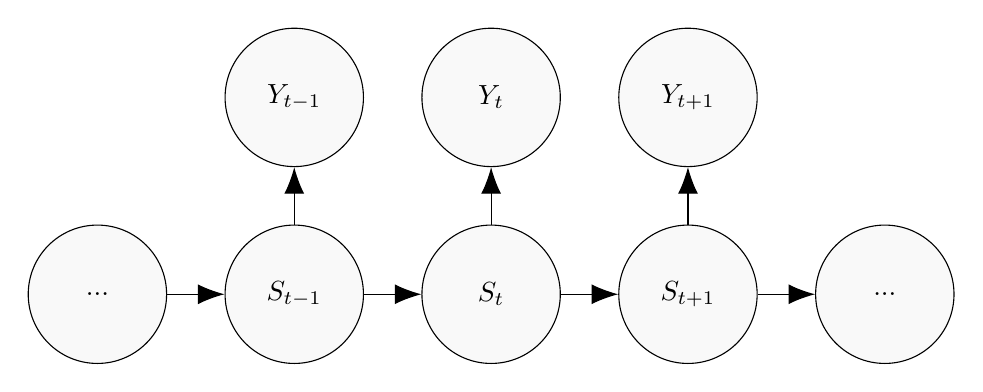
\begin{tikzpicture}
	\node[circle,draw=black, fill=gray!5, inner sep=0pt, minimum size=50pt] (A) at (2, -5) {$S_{t-1}$};
	\node[circle,draw=black, fill=gray!5, inner sep=0pt, minimum size=50pt] (A1) at (-0.5, -5) {...};
	\node[circle,draw=black, fill=gray!5, inner sep=0pt, minimum size=50pt] (B) at (4.5, -5) {$S_{t}$};
	\node[circle,draw=black, fill=gray!5, inner sep=0pt, minimum size=50pt] (C) at (7, -5) {$S_{t+1}$};
	\node[circle,draw=black, fill=gray!5, inner sep=0pt, minimum size=50pt] (C1) at (9.5, -5) {...};
	\node[circle,draw=black, fill=gray!5, inner sep=0pt, minimum size=50pt] (Y1) at (2, -2.5) {$Y_{t-1}$};
	\node[circle,draw=black, fill=gray!5, inner sep=0pt, minimum size=50pt] (Y2) at (4.5, -2.5) {$Y_{t}$};
	\node[circle,draw=black, fill=gray!5, inner sep=0pt, minimum size=50pt] (Y3) at (7, -2.5) {$Y_{t+1}$};
	\draw[-{Latex[scale=2]}] (A)--(B);
	\draw[-{Latex[scale=2]}] (B)--(C);
	\draw[-{Latex[scale=2]}] (A1)--(A);
	\draw[-{Latex[scale=2]}] (C)--(C1);
	\draw[-{Latex[scale=2]}] (A)--(Y1);
	\draw[-{Latex[scale=2]}] (B)--(Y2);
	\draw[-{Latex[scale=2]}] (C)--(Y3);
	\end{tikzpicture}
\caption{Dependence structure of the HMM used to model the defenders’ vertical positions $Y_t$, driven by the latent state variable $S_t$ that represents the currently guarded offensive player.}
\label{fig:HMM}
    \alttext{Diagram of a hidden Markov model: a chain of latent states connected by arrows over time, each state pointing to the observed lateral position of the defender at the same time point.}
\end{figure} 

% In a second step, we account for systematic heterogeneity across different defensive positions and teams. Thus, we incorporate random effects into the transition probabilities and model the transition probabilities $\gamma_{ij}$ using a mixed-effects formulation:  

% \[
% \text{logit}(\gamma_{ij}^{(p,t)}) 
% = \beta_{ij} 
% + u_{ij}^{(\text{position}[p])} 
% + v_{ij}^{(\text{team}[t])},
% \]
% where $\beta_{ij}$ represents the global fixed effect, 
% $u_{ij}^{(\text{position}[p])} \sim \mathcal{N}(0, \sigma^2_{\text{position}})$ 
% captures deviations due to the position of player $p$, 
% and $v_{ij}^{(\text{team}[t])} \sim \mathcal{N}(0, \sigma^2_{\text{team}})$ 
% accounts for team-level tendencies.  

Beyond transition dynamics, the underlying Markov chain requires an initial state distribution, denoted by $\boldsymbol{\delta}^{(1)}$, which specifies the probability of each defender guarding a particular offensive player at the beginning of time series. In many HMM applications, this initial distribution is of limited practical relevance and is often replaced by the stationary distribution of the transition probability matrix.
However, in our setting this substitution would be inappropriate, as the initial distribution in the basic, homogeneous HMM is likely to differ substantially from the stationary one. In addition, an analytic solution for the stationary distribution of a non-homogeneous HMM can only be obtained for those that include periodic components in the underlying Markov chain (\citealp{koslik2025inference}), while a hypothetical stationary distribution would differ from the real one. This is particularly severe in our case, as the initial assignments carry meaningful information since they directly influence derived summary statistics such as the number of state transitions. Consequently, misspecifying $\boldsymbol{\delta}^{(1)}$ would distort these metrics and thereby have non-negligible effects on subsequent analyses. 
A potential alternative would be to estimate the initial distribution parameters in a data-driven manner. Yet we face $5 \times M = 5 \times 4344 = 21{,}720$ distinct time series, making individual estimation infeasible. To address this issue, we determine the initial state probabilities following a best-practice approach. Specifically, we model them as a function of observed spatial relationships between defensive and offensive players: higher initial state probabilities are assigned to offensive players that are locally close to the respective defenders, serving as a proxy for initial guarding assignments. Specifically, the initial distribution is a softmax of the negative lateral distances to the five offensive players, whose sharpness parameter $\alpha$ we choose by profile likelihood. Details on the specific implementation are provided in Section~1 of the Supplementary Material.

\subsubsection{Model fitting}

We fit our hidden Markov model under a frequentist framework by directly maximizing its marginal likelihood with random effects integrated out. Specifically, letting $f$ denote a general density, $\bm{y}$ the collection of all observations, and writing model parameters as subscripts, we have the marginal likelihood function
\begin{equation}
\label{eqn:marginal_lik}
    \mathcal{L}(\bm{\theta}) = f_{\bm{\theta}}(\bm{y}) = \iiint f_{\bm{\beta}, \sigma}(\bm{y} \vert \bm{u}, \bm{v}, \bm{w}) f_{\sigma_u}(\bm{u}) f_{\sigma_{v}}(\bm{v}) f_{\sigma_{w}}(\bm{w}) \; d\bm{u} \; d\bm{v} \; d\bm{w},
\end{equation}
where $\bm{\theta} = (\beta_0, \beta_1, \sigma, \sigma_u, \sigma_v, \sigma_w)$, and $\bm{u}$, $\bm{v}$, and $\bm{w}$ are vectors of random coefficients. 
$f_{\bm{\beta}, \sigma}(\bm{y} \vert \bm{u}, \bm{v}, \bm{w})$ is the density of the data given a particular value of the random effects, i.e.\ treating them as parameters, and $f_{\sigma_u}(\bm{u})$, $f_{\sigma_{v}}(\bm{v})$, and $f_{\sigma_{w}}(\bm{w})$ are mean-zero multivariate Gaussian densities with covariance matrices $\sigma_u^2 \bm{I}$, $\sigma_v^2 \bm{I}$ and $\sigma_w^2 \bm{I}$, respectively.
Due to the structure of the conditional density of $\bm{y}$ and the dimension of $\bm{u}$, $\bm{v}$ and $\bm{w}$, the above integral is analytically intractable, and hence needs to be evaluated approximately. This can be done using the so-called \textit{Laplace approximation}. A detailed explanation is given by \citet{kristensen2016tmb}, but the core idea is to approximate the log-integrand in \eqref{eqn:marginal_lik} (for fixed $\bm{\theta}$) around its mode (in $\bm{u}$, $\bm{v}$ and $\bm{w}$) by a quadratic function. Integrating the exponential of this quadratic function results in a Gaussian integral with a closed-form solution. Constructing the approximation around the mode means that for each evaluation of the marginal likelihood, an inner optimization over $\bm{u}$, $\bm{v}$ and $\bm{w}$ has to be performed.

In practice, we only need to specify the (negative) log-integrand in \eqref{eqn:marginal_lik}, that is, the \emph{negative joint log likelihood} of the data and the random effects as an \texttt{R} function. This is just the sum of the log likelihood of the data given the random coefficients and the logarithm of the Gaussian densities of the random coefficients. Based on this function, the \texttt{R} package \texttt{RTMB} \citep{rtmb} then generates a high-performance objective function approximating the logarithm of \eqref{eqn:marginal_lik} as well as an accompanying gradient using automatic differentiation. Internally, all computations are performed in \texttt{C++}. The returned objective function can then easily be numerically maximized using standard quasi-Newton numerical optimization routines such as the one implemented in \texttt{R}'s \texttt{nlminb} \citep{gay1990usage}, by supplying the objective function and its gradient.

%\subsubsubsectionline{Computing the joint log likelihood} 
Because we include a play-specific random effect, we treat the time series of different defenders within the same play as \emph{conditionally independent} and across plays as independent. Thus, the term $\log f_{\bm{\beta}, \sigma}(\bm{y} \vert \bm{u}, \bm{v}, \bm{w})$ %--- required as an \texttt{R} function for the approach outlined above --- 
is composed of a sum of individual HMM log likelihoods for each defender's movement. % within each play. 
In order to compute such a single term, we need to marginalize over all possible state sequences that could have generated the observations, which itself is a non-trivial task. However, the summation over latent states can be efficiently computed via the well- established \textit{forward algorithm} \citep{zucchini, mews2025build}, rendering the computational complexity linear in the number of observations. The idea of this recursive scheme is that we can traverse along the time series, at each point retaining information of the likelihood up to that point as well as probabilistic information on the current state given previous observations, which is made possible by the Markov assumption \citep{lystig2002exact}.

For a defender %$i$ 
of role $r$, team $d$ in play $p$, to save ink, we write the transition probability matrix $\bm{\Gamma}^{(t,r,d,p)} = (\gamma_{ij}^{(t,r,d,p)})$ simply as $\bm{\Gamma}^{(t)}$. 
Then, the conditional likelihood (given the position-, team- and play-specific random effects) of the corresponding defender's movement can be written down in closed form as
\begin{equation}
    \label{eqn:cond_lik}
    %\mathcal{L}(\bm{\theta} \vert \bm{u}, \bm{v}, \bm{w}) =
    \bm{\delta}^{(1)} \bm{P}(y_1) \bm{\Gamma}^{(2)} \bm{P}(y_2) \bm{\Gamma}^{(3)} \dotsc \bm{\Gamma}^{(T_m)} \bm{P}(y_{T_m}),
\end{equation}
where $\bm{\delta}^{(1)}$ is the play- and defender-specific initial distribution calculated as outlined in the previous section, and $\bm{P}(y_t) = \text{diag}\bigl(f(y_t \vert S_t = 1), \dotsc, f(y_t \vert S_t = 5)\bigr)$ is a diagonal matrix containing the state-dependent distributions defined in \eqref{eqn:state_dep}.
% Time series of different defenders within the same play and of different plays are treated as independent, hence their log-likelihood contributions are summed to obtain the full likelihood of the training data. 

For practical implementation, we wrote a custom (negative joint log) likelihood function in \texttt{R}, using the function \texttt{forward\_(g)} 
% and other convenience functions 
from the \texttt{R} package \texttt{LaMa} \citep{koslikLaMa2025}, that allows evaluating the logarithm of \eqref{eqn:cond_lik} for all plays and all defenders, and thereby the computation of the term of interest $\log f_{\bm{\beta}, \sigma}(\bm{y} \vert \bm{u}, \bm{v}, \bm{w})$.

The parameters to be estimated are the two coefficients of the transition matrix, the standard deviation of the state-dependent distributions, and the three standard deviations of the random effects distributions. Due to the nature of the Laplace approximation --- performing an inner optimization over the random parameters for each outer iteration --- predicted random effects are also immediately available upon model fitting.

\subsubsection{Feature extraction from state probabilities}\label{sec:summary}
The primary objective of our unsupervised approach is to extract informative features that enhance the supervised learning models. For this, we seek to decode the underlying guarding assignments throughout the motion phase based on the observed player trajectories. HMMs are particularly suitable for this task, as they exploit both the current observations --- such as the $\mathrm{y}$-coordinates of the individual defenders and all five offensive players --- and the temporal dependencies encoded through the transition probabilities. %By leveraging information from past and future time points, the model provides a probabilistically coherent inference of matchups between defensive and offensive players over time.
While global decoding methods (e.g., the Viterbi algorithm; \citealp{zucchini}) yield the single most likely state sequence, local decoding offers a richer quantification of uncertainty.
Thus, we compute the conditional probability of each latent guarding state at each time point $t$ given the trajectories of the defender and the offensive players in that play:
$$ \Pr(S_t = j \mid y_1, \dots, y_{T_m}) $$
where $y_1, \dots, y_{T_m}$ denotes the full sequence of positional observations up to time $T_m$, $m ~=~1, \ldots, M$. This approach retains the full probabilistic information and provides a categorical state distribution for each defender at each time point $t$. %These distributions can then be summarized into interpretable statistics—such as the mean or variance of guarding probabilities or the number of state switches—which serve as informative features in our post-motion supervised models.

%To obtain both the local state probabilities and the global state sequence, we used the functions `stateprobs()` and `viterbi()` that are also contained in the R package `LaMa`.

%As we aim to retrain the supervised mod-els described above, 

To incorporate the HMM results into the supervised models, we need to transform the state decoding time series as additional features. Integrating such derived information aligns with the principle of \textit{enhanced statistical learning}, in which additional, substantively meaningful information is leveraged to improve predictive accuracy \citep{felice2025boosting}. By enriching the feature space with information derived from the HMM results, the supervised models gain access to latent dynamics that would otherwise remain unobserved. However, including the decoded state probabilities directly into the supervised learning models is not straightforward, as the state sequences constitute a multi-dimensional time series: for each defender and each time point during the motion phases, we end up with five state probabilities, one for each potential offensive skill player to be guarded. % that varies across defenders, offensive players, and time. 
To render these time series suitable for the supervised
learning framework, we derive different informative metrics that capture the essential temporal
and probabilistic characteristics of the guarding dynamics.
In earlier work, such metrics were computed from the most likely guarded offensive player at each time point. Such counts, however, ignore the uncertainty of the decoding: a defender whose assignment is ambiguous throughout the motion may obtain zero or several switches depending on small fluctuations in the data. We therefore compute all metrics as expectations under the posterior distribution of the latent state sequence given the observations, which follow from a scaled forward--backward pass \citep{zucchini}.
In particular, for each defender, we compute the expected number of switches of the guarding assignment,
\begin{equation}\label{eq:decod}
E_{\text{sw}} = \sum_{t=2}^{T_m} \Pr(S_t \neq S_{t-1} \mid y_1, \dots, y_{T_m}) = \sum_{t=2}^{T_m} \Bigl(1 - \sum_{k=1}^{5} \Pr(S_{t-1} = k, S_t = k \mid y_1, \dots, y_{T_m})\Bigr),
\end{equation}
as well as the probability that the defender switches at least once during the motion phase, $1 - \sum_{k=1}^{5} \Pr(S_1 = \dots = S_{T_m} = k \mid y_1, \dots, y_{T_m})$. Summing over the five defenders of a play yields the expected total number of switches within a play and the expected number of defenders who switch between offensive players at least once in the respective play.
In addition to these metrics, we compute a statistic reflecting the uncertainty in the guarding assignments. Specifically, we calculate the (defensive) mean entropy across defenders $j = 1, \ldots, 5$ within each play $m = 1, \ldots, M$ (see \citealp{franks2015}) as
\[
H(m) = -\frac{1}{5} \sum_{j_m=1}^{5} \sum_{k=1}^{5} \bar{p}_{k,j_m} \log \bar{p}_{k,j_m}, \qquad \bar{p}_{k,j_m} = \frac{1}{T_m} \sum_{t=1}^{T_m} \Pr(S_{t,j_m} = k \mid y_{1,j_m}, \dots, y_{T_m,j_m}),
\]
where $S_{t,j_m}$ denotes the state of the $j$-th defender in play $m$, i.e., the entropy of the time-averaged state probabilities.

Entropy, as a measure of uncertainty in a probability distribution, provides insight into the consistency of the defensive assignments: Lower entropy values indicate stable and predictable defensive structures, whereas higher values reflect increased variability and uncertainty in matchups. 

Finally, we also incorporate the estimated play-specific random effect --- which captures overarching tendencies to switch the guarding assignment in that respective play --- as an additional feature (see Eq.~\ref{eq:re}).

\subsection{Supervised learning}
Our supervised learning approach aims to predict the defensive coverage type --- man or zone --- based on several features. %As our dataset comprises only \( M = 3985 \) passing plays that include pre-snap motion, model complexity must be carefully controlled to avoid overfitting. %Since the main focus of this paper is the incorporation of features describing pre-snap motion, 
For this, we follow a three-step approach: First, we establish a baseline model for coverage type prediction using only the contextual and spatial pre-motion features derived in Section~\ref{sec:data}. This model serves two purposes. On the one hand, it provides a natural baseline for comparing models using motion information. On the other hand, this model is useful when analysing the impact of using motion to detect the correct coverage scheme (see Section \ref{sec:team_analysis}). Second, we fit a model to an augmented set of features containing naive post-motion information derived in Section~\ref{sec:data}. Third, we fit a model using both the pre-motion and naive post-motion features and additionally the previously described HMM features. This enriched model therefore contains directly observable post-motion information but also latent assignment patterns inferred from the HMM, thereby capturing relevant dynamics of the defensive coverage.

To model the probability that a play \( i \in \{1, \dots, M\} \) corresponds to a man (\( y_i = 1 \)) or zone (\( y_i = 0 \)) coverage, we fit two complementary model classes: an elastic net logistic regression \citep{Zou05elastic} and gradient-boosted decision trees, implemented as an XGBoost model \citep{chen2016xgboost}. The former model is an interpretable model known to handle large feature spaces by regularization and implicit variable selection. However, its strong modelling assumptions, particularly the assumption of linear relationship between features and log odds of the outcome, may limit predictive performance. The latter is more flexible, allowing for non-linearities and interactions between features, at the cost of interpretability. Furthermore, tree boosting models typically require a large amount of data for proper hyperparameter tuning. In \texttt{R}, we use the \texttt{glmnet} \citep{friedman2021package} and the \texttt{xgboost} \citep{chen2019package} packages.

\subsection{Model evaluation and inference}
\label{sec:model_eval}
There are various objectives when evaluating the performance of our three-step supervised learning approach described in the previous section. One aim is to obtain a well-performing model for predicting the coverage type. That is, we want to compare the performance of the three models on a set of unseen data points. Commonly used loss metrics for a binary outcome are accuracy, i.e., the percentage of correctly classified observations; the area under the receiver operating characteristic curve (AUC), i.e., the area under the mapping between the true positive rate (TPR) and the false positive rate (FPR); %, or equivalently, the probability that the model ranks a randomly chosen positive instance higher than a randomly chosen negative instance, 
and the logloss, i.e., the (negative) log-likelihood value. For both the elastic net and the XGBoost model this coincides with a Bernoulli log-likelihood based on the predicted probability for each observation. 
The most popular loss metric is arguably the accuracy due to its simple interpretation. However, evaluating performance on accuracy can be misleading as it is dependent on the threshold selected for classification of the outcome \citep[see, e.g.,][]{tholke23acc}. Typically, for probabilistic predictions, as obtained by the two model classes considered, one uses the naive threshold of $0.5$. The AUC, on the other hand, is threshold independent as it compares TPR and FPR among a range of possible values. Hence, it is more suitable for binary classification, especially in imbalanced setups. From a mathematical perspective, the logloss is the most attractive loss metric due to being a proper scoring rule \citep{waghmare25scoring}, i.e., it is maximized in expectation by the true probabilities of each class. Hence, in this work, we mainly focus on the logloss to evaluate model performance, but for reasons of comparison, we also indicate the other loss metrics. 

While evaluating predictive performance on hold-out data allows for identifying the best-performing models, it is not suitable for inference on the features. More specifically, an important question is to identify which features are significantly associated with the outcome. %Or, in our case, we are interested in testing whether the 
In many fields, including sports analytics, the identification of influential factors is often approached by fitting machine learning models and examining traditional variable importance measures \citep{bajons2025mlsi}. However, variable importance measures differ by the regression technique used, hence do not allow for comparison between regression models \citep{williamson20varimp}. Additionally, there are various ways to compute variable importance measures for tree ensembles as used in this work, each having its own advantages and disadvantages \citep{Strobl08varimp}. A recently popularized alternative are non-parametric conditional independence tests. As opposed to traditional variable significance tests, which assume a parametric relationship between outcome and features, these tests determine which features are significantly associated with an outcome with considerably relaxed assumptions, generally relying on modern machine learning algorithms. In this work, we consider a popular family of such tests commonly referred to as covariance measure tests \citep[COMETs, see, e.g.,][]{kook24comets}, and specifically, the Generalized Covariance Measure (GCM) test \citep{Shah20gcm}. COMETs test for conditional independence of an outcome variable $Y$ and a (possibly vector-valued) feature $X$ given additional features $Z$, without imposing strong (parametric) assumptions on the (conditional) distribution of $Y$.
More formally, the GCM test assesses the conditional independence of $Y$ and $X$ given $Z$, denoted by $Y \perp\!\!\!\perp X \mid Z$, by targeting the 
\begin{equation}\label{eq:GCM}
\operatorname{GCM} \coloneqq \mathbb{E}[\operatorname{Cov}(Y,X \mid Z)] =\mathbb{E}[(Y -
\mathbb{E}[Y | Z])(X - \mathbb{E}[X | Z])],
\end{equation}
and using the fact that a necessary condition for $Y \perp\!\!\!\perp X \mid Z$ is that $\mathbb{E}[\operatorname{Cov}(Y,X \mid Z)] = 0$. To obtain an empirical estimate of the GCM, one therefore has to learn two regression functions $h(Z) \coloneqq \mathbb{E}[Y | Z]$ and $f(Z) \coloneqq \mathbb{E}[X | Z]$. The test remains valid under mild assumptions, which are typically met when these functions are estimated by suitable machine learning methods \citep{Shah20gcm}, and thus remains applicable even without imposing strong modelling assumptions.
% Hence, these tests can be used even when modelling the outcome with modern machine learning algorithms. 
Aside from its statistical merit, the GCM test is also appealing from an interpretational viewpoint. \citet{bajons2025rGAX} show that for a binary outcome, as in our case, the GCM test can be related to a parameter estimate in semi-parametric partially linear logistic regression model.
More precisely, let $(Y, X, Z)$, where $Y \in \{0, 1\}$, $X \in \mathbb{R}^{d_X}$, $Z \in \mathbb{R}^{d_Z}$, be a random vector in which $Y$ is governed by a partially linear regression model. That is, $Y \given X, Z \sim \operatorname{Ber}(\pi(X,Z))$
follows a Bernoulli distribution with $\pi(X,Z) = P(Y=1 \mid X,Z) = \mathbb{E}[Y \given
X,Z]$, and 
\begin{align}
\label{eq:pllm_lo}
\begin{aligned}
\log\left(\frac{\pi(X,Z)}{1-\pi(X,Z)}\right) =
X\beta + g(Z),
\end{aligned}
\end{align}
with some arbitrary measurable function $g$. Then, \citet{bajons2025rGAX} show that the GCM test can be used to test hypotheses of the form $H_0: \beta = 0$ as well as $H_0 \ge 0$ (respectively $H_0 \le 0$) in the PLLM.  
That is, using the GCM test, we can not only identify which feature is significantly associated with the outcome, but also interpret the direction that a feature influences it in the context of the model from Eq.~\ref{eq:pllm_lo}. In our case, we use the GCM test implemented in \texttt{R} via the \texttt{comets} package (\citealp{kook24comets}) to assess whether HMM-derived features significantly influence man-versus-zone predictions after conditioning on all other variables, including naive post-motion features. Additionally, we interpret the results of the tests within the partially linear logistic regression model of Eq.~\ref{eq:pllm_lo}.

\section{Results}\label{sec:results}
In this section, we first present results from the hidden Markov model (HMM), including estimated transition dynamics, random effects, and decoded state probabilities that capture latent guarding assignments. We then report results from supervised learning models predicting defensive coverage schemes. Next, we evaluate whether the additional HMM-derived features yield statistically significant improvements in predictive performance. Finally, we demonstrate the practical utility of our framework through team-level analyses.

\subsection{Unsupervised learning}
Before fitting the full HMM incorporating random effects in its state process, we first estimated a simpler version with a homogeneous Markov chain to determine the optimal time lag $l$ corresponding to defenders’ reaction times (see Eq. \ref{eq:lag}). The table in Section~2 of the Supplementary Material shows that lags of $l = 4$ and $l = 5$ are clearly preferred over shorter and longer lags according to AIC values, while the two are nearly indistinguishable. This aligns closely with previously reported reaction times in soccer (\citealp{wu2023evaluation}). We use $l = 4$ when fitting our full model. Similarly, the profile likelihood of the sharpness parameter of the initial distribution is maximal at $\alpha = 4$ (Section~1 of the Supplementary Material).

Table~\ref{tab:fixed} reports the estimated parameters of the full model. Guarding assignments are highly persistent ($\hat\beta_0 = -2.99$), and switches are much more likely between offensive players who are close to each other: each yard of lateral distance multiplies the odds of a switch by $\exp(\hat\beta_1) = 0.43$. The variance components show that plays differ much more in their switching tendency than defensive teams or positions.

\begin{table}[t!]
\centering
\caption{Estimated parameters of the HMM with standard errors and 95\% confidence intervals (for the standard deviations obtained on the log scale).}
\label{tab:fixed}
\begin{tabular}{lrrr}
\hline
Parameter & Estimate & Std.\ error & 95\% CI \\
\hline
$\beta_0$ (intercept) & $-2.993$ & 0.069 & $[-3.128, -2.858]$ \\
$\beta_1$ (distance, per yard) & $-0.853$ & 0.011 & $[-0.874, -0.832]$ \\
$\sigma$ (yards) & 1.911 & 0.001 & $[1.908, 1.913]$ \\
$\sigma_{\text{role}}$ & 0.142 & 0.042 & $[0.080, 0.254]$ \\
$\sigma_{\text{defense}}$ & 0.117 & 0.024 & $[0.079, 0.174]$ \\
$\sigma_{\text{play}}$ & 0.546 & 0.021 & $[0.505, 0.589]$ \\
\hline
\end{tabular}
\end{table}

The most intriguing results --- apart from the decoded state sequences --- relate to the estimated transition probability matrix, which includes the random effects. Table~\ref{tab:position_effects} summarizes the predicted random effects across positions. These effects quantify how state-switching probabilities vary by role. Smaller values correspond to a higher likelihood of remaining in the current state, i.e., continuing to guard the same offensive player at subsequent time steps. Consistent with visual observation, cornerbacks exhibit strong tendencies to follow receivers across plays, whereas linebackers most frequently pass off coverage assignments; safeties lie in between.

\begin{table}[b!]
\centering
\caption{Predicted random effects separated for each defensive position, with prediction standard errors.}
\label{tab:position_effects}
\begin{tabular}{lrr}
\hline
Position & Predicted Effect & Std.\ error \\
\hline
Inside Linebacker & $\ \ \ 0.182$ & 0.065 \\
Middle Linebacker & $\ \ \ 0.153$ & 0.081 \\
Outside Linebacker & $\ \ \ 0.224$ & 0.071 \\
Cornerback & $-0.207$ & 0.064 \\
Strong Safety & $\ \ \ 0.112$ & 0.075 \\
Free Safety & $-0.038$ & 0.076 \\
\hline
\end{tabular}
\end{table}

Similarly, Section~4 in the Supplementary Material displays the predicted random effects for all defensive teams. These estimates reflect structural differences in defensive schemes between teams. 

The position-, team-, and play-level random effects are incorporated into the overall state-switching dynamics of the HMM. Since the underlying Markov chain is modelled in a non-homogeneous manner, it is not possible to present a single transition probability matrix. Nevertheless, to provide intuition regarding the state transitions, we report the estimated transition probability matrix (t.p.m.) for Marco Wilson, a cornerback of the Arizona Cardinals, in the play shown in Figure~\ref{fig:prepro}. Specifically, this t.p.m.\ corresponds to the moment when Mecole Hardman (MH) --- the player Marco Wilson is covering --- crosses running back Jerick McKinnon (JMK). This example demonstrates the strength of our approach: although Wilson is momentarily as close to McKinnon as to Hardman, his estimated tendency to stay with Hardman remains high (see $\hat{\gamma}_{11}$), reflecting realistic persistence in man‑to‑man coverage behaviour.

$$
\renewcommand{\arraystretch}{1.2}
\setlength{\arraycolsep}{4pt}
\begin{array}{c|c}
    &
\hspace{-0.8em} % etwas nach links schieben
    \begin{array}{ccccc}
        \ \ \ \ \ \ \text{MH} \ \ \ \ & \text{TK} \ \ \ & \text{JMK} \ \ \ & \text{JSS} \ \  & \text{MVS}\ \ 
    \end{array}
    \hspace{-1em} % etwas nach rechts schieben
    \\[4pt] \hline
    \begin{array}{c}
        \text{MH} \\[1pt] 
        \text{TK} \\[1pt]
        \text{JMK} \\[1pt]
        \text{JSS} \\[1pt]
        \text{MVS} 
    \end{array}
    &
    \left(
      \begin{array}{ccccc}
      0.974 & 0.001 & 0.025 & 0.000 & 0.000 \\
      0.001 & 0.998 & 0.001 & 0.000 & 0.000 \\
      0.025 & 0.001 & 0.974 & 0.000 & 0.000 \\
      0.000 & 0.000 & 0.000 & 1.000 & 0.000 \\ 
      0.000 & 0.000 & 0.000 & 0.000 & 1.000
      \end{array}
    \right)
\end{array}
$$

Overall, estimated transition probabilities indicate largely stable and persistent latent-state dynamics. Occasionally elevated state-switching probabilities (such as $\hat{\gamma}_{13}$) occur when defenders move toward offensive players occupying similar horizontal zones (e.g., JMK). In contrast, transitions to more distant offensive targets (Travis Kelce, TK; Juju Smith-Schuster, JSS; or Marquez Valdes-Scantling, MVS) are seldom observed.

\begin{figure}
    \centering
    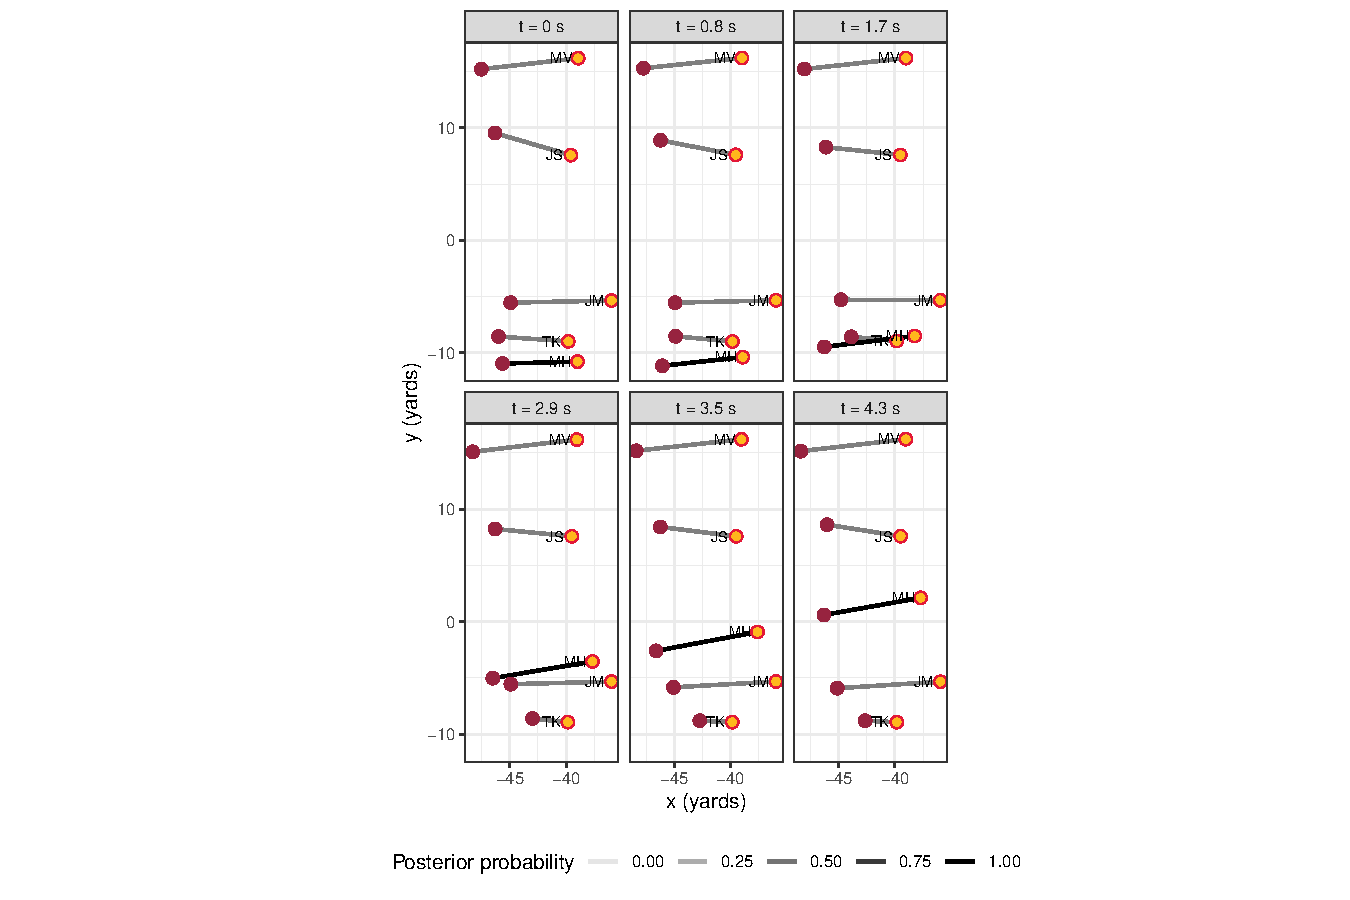
\includegraphics[width=\linewidth]{figures/plots/snapshot.pdf}
    \caption{This figure illustrates how guarding assignments evolve during an example play based on the local state probabilities from our HMM analysis. Lines between offensive and defensive players represent inferred matchups over time. The top-left panel shows initial formations at the line of scrimmage; subsequent panels depict intermediate stages culminating in the bottom-right frame immediately before the snap. Notably, when Mecole Hardman (MH) crosses paths with running back Jerick McKinnon (JMK), Marco Wilson’s coverage remains firmly maintained on Hardman.}
    \label{fig:snap}
    \alttext{Six snapshots of an example play showing defenders and offensive players on the field; lines between them, whose opacity reflects the posterior probability of the guarding assignment, show that the cornerback Marco Wilson keeps guarding Mecole Hardman when Hardman crosses another offensive player.}
\end{figure}


\begin{table}[!t]
\caption{Summary statistics of the features that were extracted from the posterior state probabilities.}
\label{tab:state_decod}
\centering
\begin{tabular}[t]{lrrrr}
\hline
statistic & Exp.\ total switches & Exp.\ \# switching defenders & avg.\ entropy & RE/play\\
\hline
Min. & 0.00 & 0.00 & 0.00 & -1.04\\
1st Qu. & 0.37 & 0.32 & 0.04 & -0.17\\
Median & 1.77 & 1.42 & 0.16 & -0.03\\
Mean & 2.12 & 1.54 & 0.20 & 0.00\\
3rd Qu. & 3.11 & 2.27 & 0.29 & 0.17\\
Max. & 16.81 & 5.00 & 0.91 & 1.26\\
\hline
\end{tabular}
\end{table}

While these results offer valuable insights into latent state-switching dynamics, our main focus lies in the state probabilities and their translation into the summary statistics described above. As an example, Figure~\ref{fig:snap} illustrates how the HMM effectively captures Marco Wilson's guarding assignment\footnote{A complete animation of the sequence is provided as supplementary material.}. Interestingly, the unique strength of HMMs becomes apparent when Wilson reaches the same $\mathrm{y}$-coordinate as running back Jerick McKinnon. At this moment, the HMM consistently and accurately maintains the correct coverage assignment throughout the motion as a consequence of its temporal persistence. In contrast, classical clustering algorithms based solely on spatial proximity, ignoring the temporal dependencies, would likely suggest a change in guarding assignment, thereby introducing noise. 

We transformed the state probabilities into the metrics described in Section~\ref{sec:summary}. Table~\ref{tab:state_decod} summarizes key descriptive statistics such as the minimum, maximum and mean of the expected number of state switches, the expected number of defenders who change their guarding assignment throughout the motion phase, the defensive mean entropy across defenders and the predicted random effect per play. As posterior expectations, the first two are not restricted to integers. On average, plays in man coverage show fewer expected switches (1.85 vs.\ 2.22 in zone coverage), fewer switching defenders (1.30 vs.\ 1.62) and a lower mean entropy (0.17 vs.\ 0.21).

\subsection{Supervised learning}

\begin{figure}
    \centering
    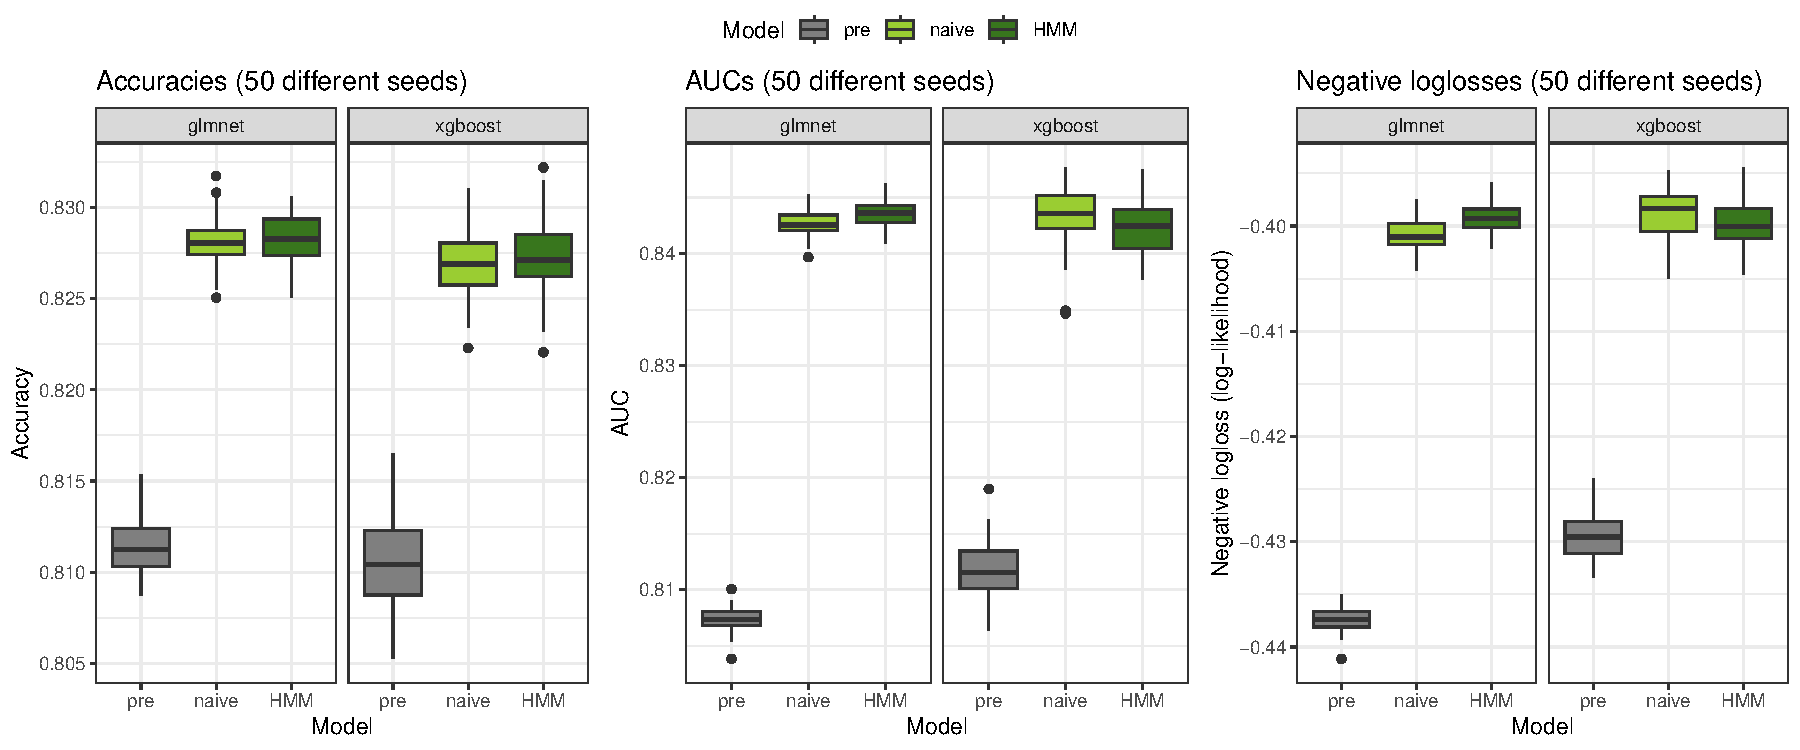
\includegraphics[width=\linewidth]{figures/plots/all_losses_cross_fitting.pdf}
    \caption{Top: Boxplots of the different loss metrics (left subpanel: accuracies; middle: AUC; right: negative logloss) obtained from 50 different runs of the cross fitting procedure. Each panel contains the results from the elastic net (\texttt{glmnet}) on the left and the XGBoost model, on the right. Bottom: Paired differences between the models with HMM features and with naive post-motion features for each run (points), on separate scales; positive values indicate an improvement by the HMM features.}
    \label{fig:loss_metrics}
    \alttext{Top row: boxplots of accuracy, AUC and negative logloss for the pre-motion, naive post-motion and HMM models, separately for elastic net and XGBoost; the pre-motion models are clearly worst. Bottom row: boxplots of the paired differences between HMM and naive models per run; for the elastic net, all differences in AUC and negative logloss are positive, for XGBoost they scatter around zero.}
\end{figure}

As described in Section \ref{sec:model_eval}, we first compare the performance of the baseline model using only pre-motion features with the model using additional naive post-motion features, % (denoted by ``naive''), 
and the model using all previous features and the HMM-derived features. % (denoted by \textit{HMM}). 
Since we are working with a small data set, we implement a cross-fitting strategy to obtain out-of-sample predictions for each observation. Specifically, we randomly split the full data into five folds. For each fold, we train a model on all data except the data contained in the selected fold.  Both model classes --- the elastic‑net and XGBoost models --- require specification of hyperparameters; therefore, within each training iteration we perform 5‑fold cross-validation on the remaining four folds to tune these parameters. More precisely, we use a pre-defined grid to tune \( \lambda \) and $\alpha$ for the elastic net, and tree depth, learning rate, column subsampling rate, minimum loss reduction for a split, and number of boosting rounds for XGBoost. The tuned models are then used to generate predictions for all observations in the left-out fold. Repeating this procedure yields out-of-sample predictions for every play in the data set. Hereby, we can compare our three models using the different loss metrics (accuracy, AUC, and logloss) on unseen data. However, because cross‑fitting involves random partitioning into five folds and further random splits during inner cross-validation for hyperparameter tuning, estimates of out‑of‑sample losses may vary depending on these random draws. To address this source of uncertainty, we repeat the entire cross-fitting routine 50 times and report resulting distributions of loss metrics rather than a single value from one random split. Since all models are evaluated on the same partitions, we compare them by paired differences.

%For both models, we conduct 10-fold cross-validation over a pre-defined hyperparameter grid to identify optimal values of \( \lambda \) and $\alpha$ (for the logistic elastic net), as well as tree depth, learning rate, and number of boosting rounds (for the XGBoost model).

Figure~\ref{fig:loss_metrics} and Table~\ref{tab:perf} display the results of the cross-fitting loss evaluation procedure, and Table~\ref{tab:paired} the paired differences between the models. Both model classes perform very similarly. The pre-motion models perform worst, suggesting that even a naive incorporation of motion information substantially improves prediction of the defensive coverage scheme: in every run, the naive post-motion features reduce the logloss by about 0.036 (elastic net) and 0.031 (XGBoost), and increase the AUC by about 0.035 and 0.032 and the accuracy by about 1.7 and 1.6 percentage points, respectively. Including HMM-derived features further improves the elastic net slightly but consistently (logloss $-0.0015$ and AUC $+0.0009$ in all 50 runs), whereas its accuracy is virtually unchanged. For XGBoost, in contrast, the HMM features do not improve the predictions (logloss $+0.0009$ on average, lower in 18 of 50 runs), so that the elastic net with HMM features and the XGBoost model with naive post-motion features reach the same logloss of 0.399. Hence, much of the information that the HMM features carry about the coverage scheme is already contained in simpler summaries of the motion. With $M = 4344$ plays and a minority class of 25\%, however, out-of-sample loss metrics are a coarse instrument to detect a weak but genuine signal, as any gain is small relative to the variance that additional features introduce, in particular for flexible learners such as XGBoost. We therefore assess more directly whether the HMM features carry information about the coverage scheme that is not contained in the other features.

\begin{table}[t!]
\centering
\caption{Out-of-sample loss metrics (mean and, in brackets, standard deviation over 50 runs of the cross-fitting procedure) of the models with pre-motion features (pre), pre- and naive post-motion features (naive), and additionally the HMM features (HMM).}
\label{tab:perf}
\begin{tabular}{llccc}
\hline
Model & Features & Accuracy & AUC & Logloss \\
\hline
Elastic net & pre & 0.812 (0.002) & 0.807 (0.001) & 0.437 (0.001) \\
 & naive & 0.828 (0.001) & 0.843 (0.001) & 0.401 (0.001) \\
 & HMM & 0.828 (0.001) & 0.844 (0.001) & 0.399 (0.001) \\
XGBoost & pre & 0.811 (0.002) & 0.812 (0.003) & 0.430 (0.002) \\
 & naive & 0.827 (0.002) & 0.843 (0.003) & 0.399 (0.002) \\
 & HMM & 0.827 (0.002) & 0.842 (0.002) & 0.400 (0.002) \\
\hline
\end{tabular}
\end{table}

\begin{table}[t!]
\centering
\caption{Paired differences between the models over the 50 runs of the cross-fitting procedure: mean and, in brackets, 2.5\% and 97.5\% quantiles. Positive differences in accuracy and AUC and negative differences in the logloss indicate an improvement.}
\label{tab:paired}
\begin{tabular}{llcc}
\hline
Model & Metric & naive $-$ pre & HMM $-$ naive \\
\hline
Elastic net & Accuracy & 0.0166 [0.0127, 0.0197] & 0.0002 [$-$0.0027, 0.0037] \\
 & AUC & 0.0354 [0.0339, 0.0366] & 0.0009 [0.0002, 0.0015] \\
 & Logloss & $-$0.0365 [$-$0.0379, $-$0.0351] & $-$0.0015 [$-$0.0022, $-$0.0009] \\
XGBoost & Accuracy & 0.0163 [0.0102, 0.0213] & 0.0002 [$-$0.0027, 0.0035] \\
 & AUC & 0.0319 [0.0273, 0.0372] & $-$0.0011 [$-$0.0044, 0.0030] \\
 & Logloss & $-$0.0307 [$-$0.0357, $-$0.0269] & 0.0009 [$-$0.0029, 0.0047] \\
\hline
\end{tabular}
\end{table}

\begin{figure}
    \centering
    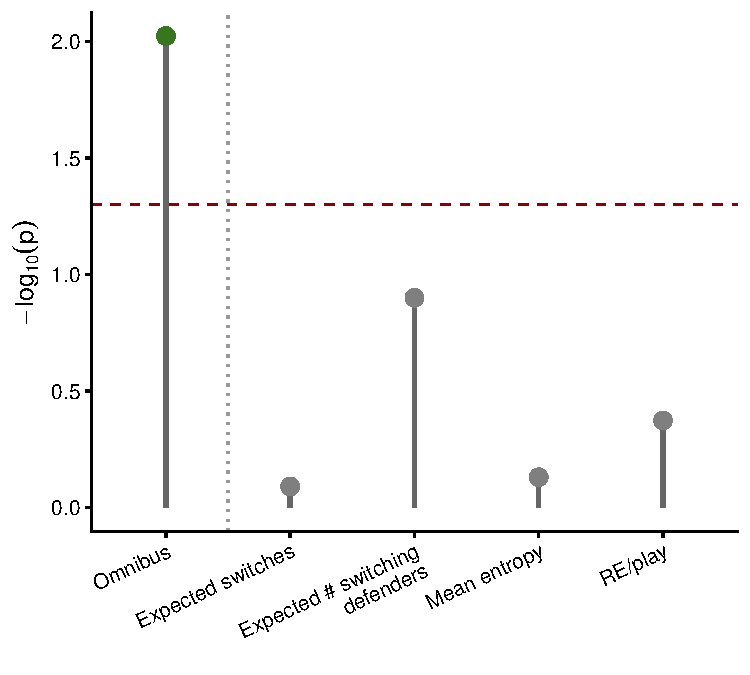
\includegraphics[width=0.5\linewidth]{figures/plots/gcm_test_all_plus_omnibus.pdf}
    \caption{$p$-values on a $-\log_{10}$-scale of the GCM test for conditional independence of HMM features and coverage outcome given pre- and naive post motion features as well as all other HMM features for the individual tests. The dashed horizontal line indicates the 5\%-level. The dotted vertical line separates the omnibus test, i.e., a test on all features simultaneously from the tests on specific features.}
    \label{fig:sig1}
    \alttext{Lollipop chart of minus log10 p-values of the partial GCM tests; only the omnibus test exceeds the line of the 5 percent level, the four individual features lie below it.}
\end{figure}

Further evidence of the usefulness of the HMM-derived features comes from the GCM test described in Section~\ref{sec:model_eval}. This test allows us to statistically assess whether these features carry information on the coverage scheme beyond the other features. For this analysis, we used the XGBoost model, as the regression method for the estimation of $h(Z)$ and $f(Z)$ (see Section~ \ref{sec:model_eval}). More specifically, the GCM test can be applied in several ways. Let $X \in \mathbb{R}^4$ denote the set of HMM features; we first test the null hypothesis $Y \perp\!\!\!\perp X \mid Z$, i.e., we perform an omnibus test, which assesses whether at least one of the HMM-derived features is significantly associated with the defensive coverage outcome $Y$. The result of this test is shown in Figure \ref{fig:sig1}. The test is significant at the 1\% level ($p$-value $\approx 0.009$), indicating that the HMM-derived features carry information on the defensive coverage scheme even in the presence of pre- and naive post-motion features. Next, we test for each feature in $X$ individually, i.e., perform a test of the form $H_0^j: Y \perp\!\!\!\perp X_j \mid (Z,X_{-j})$, $j = 1,\dots,4$, where $-j$ denotes the set of features when removing feature $j$. Figure~\ref{fig:sig1} demonstrates that none of the features is significant individually given the other three ($p$-values between 0.13 and 0.81). While this result may seem surprising, it is most likely explained by strong correlation among the HMM features: together they carry information, but each can largely be replaced by the others. 

\begin{figure}
    \centering
    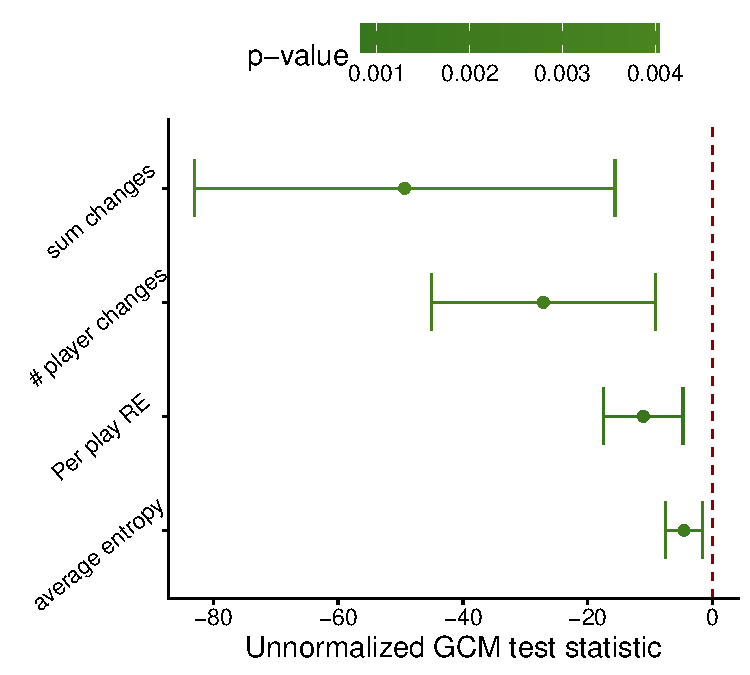
\includegraphics[width=0.5\linewidth]{figures/plots/gcm_teststat.pdf}
    \caption{Normalized statistics of the GCM tests of each HMM feature given the pre- and naive post-motion features. Dashed lines: two-sided critical values at the 5\%-level; dotted lines: Bonferroni-corrected critical values for four tests.}
    \label{fig:sig2}
    \alttext{Lollipop chart of the normalized marginal GCM test statistics of the four HMM features; all four are negative, between about minus 2.9 and minus 3.3, and beyond both the 5 percent and the Bonferroni-corrected critical values.}
\end{figure}


To gain deeper insight into the individual HMM-derived features, we analyse them within the framework of the partially linear logistic regression model defined in Eq.~\ref{eq:pllm_lo}. To this end, we consider each feature $X_j$ individually. More precisely, we test the hypotheses $H_0^j: Y \perp\!\!\!\perp X_j \mid Z$, $j = 1,\dots,4$, i.e., given the pre- and naive post-motion features only, which corresponds to testing $H_0: \beta = 0$ in a partially linear logistic regression model for $(Y,X_j,Z)$. Figure~\ref{fig:sig2} shows the resulting normalized GCM test statistics for each feature. First, we observe that all features are significant, also after a Bonferroni correction for four tests ($p$-values between 0.0008 and 0.004). Second, the test statistics are negative for all HMM-derived features (see Figure~\ref{fig:sig2}). This implies that the coefficient $\beta$ in Eq.~\ref{eq:pllm_lo} is significantly negative, indicating a negative effect of all features on the probability of man coverage. This finding aligns with our intuition. Lower values of the features describing the number of switches and the total count of assignment changes indicate lower variability in latent guarding patterns, typically a characteristic of man coverage. The average entropy is somewhat more complex to interpret but conceptually similar to these two metrics; hence its significantly negative impact on coverage outcome appears equally reasonable. The estimated random effect from the HMM model that we include as a feature is different in nature to the previous three. It influences transition probabilities of the latent Markov chain (see Section \ref{sec:MC_dets}). A higher estimate corresponds to an increased probability of switching states, which in turn represents changes in latent guarding assignments. Hence, the strongly negative impact on the probability of man coverage is also reasonable in this case.

The significant tests and the small predictive gains are consistent with each other. A normalized GCM statistic $T$ corresponds approximately to a correlation of $T/\sqrt{M}$ between the residuals $Y - \mathbb{E}[Y \mid Z]$ and $X_j - \mathbb{E}[X_j \mid Z]$. With $|T| \approx 3$ and $M = 4344$, this partial correlation is about $0.045$, i.e., each HMM feature explains only about $0.2\%$ of the residual variation of the coverage scheme. In a logistic model, a feature with partial correlation $\rho$ reduces the expected logloss by roughly $\rho^2/2$, here about $0.001$, which matches the improvement of the elastic net. While the test statistic grows with $\sqrt{M}$, so that such a weak association is detectable with our sample size, the predictive gain is of the order of $\rho^2$ and is easily offset by the estimation error of additional features, in particular for flexible learners such as XGBoost that approximate a weak monotone effect by many estimated splits.


\subsection{Team analysis}
\label{sec:team_analysis}

\begin{figure}
    \centering
    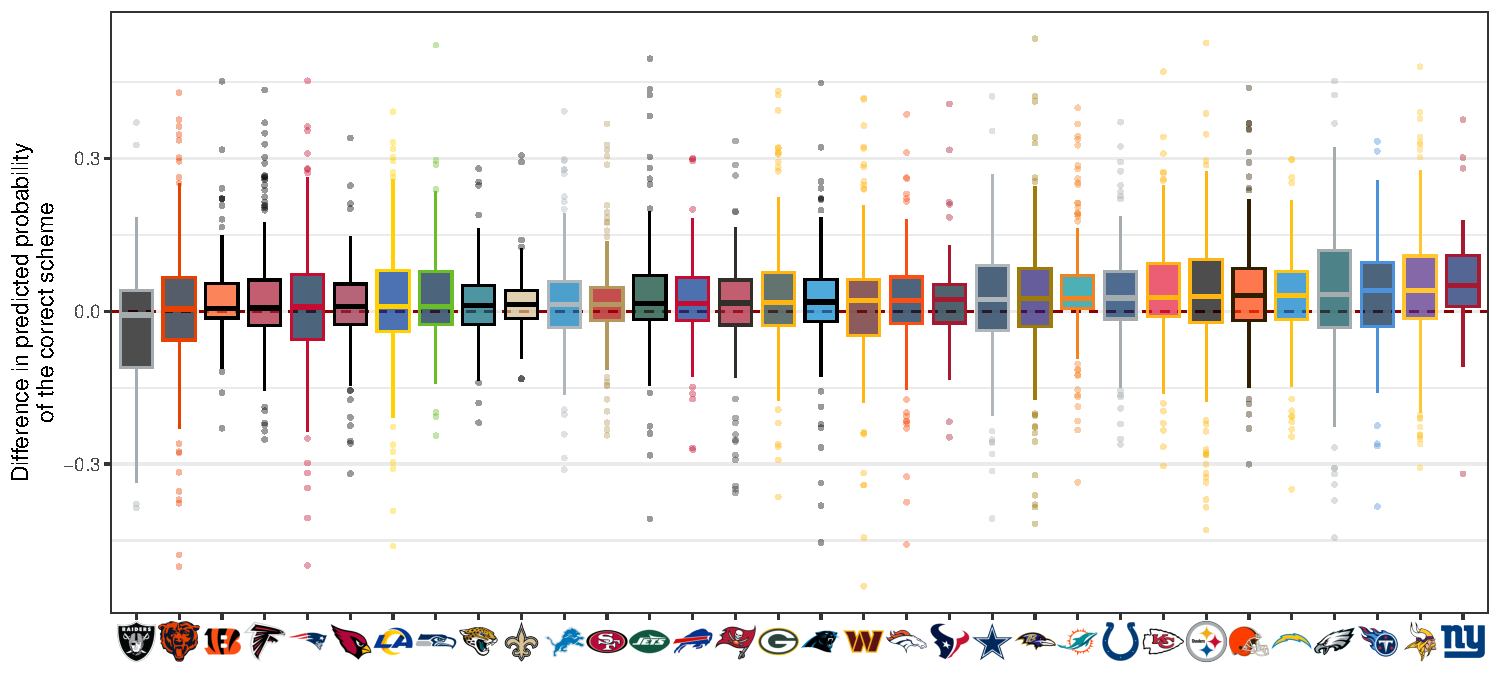
\includegraphics[width=\linewidth]{figures/plots/team_diffs.pdf}
    \caption{Boxplots of the differences in the predicted probability of the correct defensive scheme between a model using motion features and a model using only pre motion features for each play of each team in the NFL. Teams are ordered by medians of the boxplots.}
    \label{fig:teamdiff}
    \alttext{Boxplots of the per-play differences in the predicted probability of the correct scheme for each of the 32 offenses, ordered by their medians, which are mostly slightly above zero.}
\end{figure}

While this study primarily focuses on play-level predictions of defensive coverage schemes, the coverage models can also be used to evaluate teams’ ability to use pre‑snap motion to identify the correct coverage, assuming that their visual identification aligns with our statistical forecasts.  

\begin{table}[t!]
\centering
\caption{Number of motion plays, number of plays where the motion improved the probability of predicting the correct outcome, and proportion of motion plays where the probability of the correct outcome was improved (with Wilson 95\% confidence interval) for the top ten NFL teams with respect to improvement percentage.}
\label{fig:team_tab}
\begin{tabular}{llrrr}
\hline
 & Team & Motion plays & Improved & Proportion [95\% CI] \\
\hline
1 & New York Giants & 63 & 52 & 0.83 [0.71, 0.90] \\
2 & Miami Dolphins & 244 & 190 & 0.78 [0.72, 0.83] \\
3 & Minnesota Vikings & 176 & 127 & 0.72 [0.65, 0.78] \\
4 & Los Angeles Chargers & 159 & 112 & 0.70 [0.63, 0.77] \\
5 & Kansas City Chiefs & 170 & 116 & 0.68 [0.61, 0.75] \\
6 & Cleveland Browns & 140 & 95 & 0.68 [0.60, 0.75] \\
7 & Indianapolis Colts & 124 & 84 & 0.68 [0.59, 0.75] \\
8 & Denver Broncos & 135 & 91 & 0.67 [0.59, 0.75] \\
9 & Pittsburgh Steelers & 144 & 97 & 0.67 [0.59, 0.74] \\
10 & Houston Texans & 81 & 54 & 0.67 [0.56, 0.76] \\
\hline
\end{tabular}
\end{table}

To assess how effectively teams utilize pre-snap motion to recognize defensive coverage schemes, we compare predictions from two of the three supervised models: the pre-motion XGBoost model and the post-motion XGBoost model including HMM features. For estimation, we adopt an out-of-sample prediction strategy to avoid data leakage between training and evaluation phases. Specifically, for each team under consideration, all plays belonging to that team are excluded during model training and hyperparameter tuning. Afterwards, the two models are trained on data from all remaining teams using cross-validation procedures described earlier. Predictions for the omitted team’s plays are then generated using these fitted models. Although this leave-one-team-out procedure may not exploit intra-team characteristics optimally due to data limitations, it ensures unbiased performance assessment across teams. We then evaluate the corresponding predicted probabilities of correct classification obtained from both models. Conceptually, if pre-snap motion assists offenses in recognizing defensive structures, predictions from the model including motion should yield higher probabilities than those from the model without motion.
Figure~\ref{fig:teamdiff} visualizes these differences using boxplots for each team, ordered by their median improvement values. The results reveal considerable variation across teams but generally indicate positive median differences, suggesting that most teams benefit from motion-based information when anticipating coverages. Overall, the probability of the correct scheme increases in 63\% of the motion plays, and for all teams except the Las Vegas Raiders in more than half of their motion plays.

Complementary insights are provided by Table~\ref{fig:team_tab}, which lists the ten teams with the largest proportion of plays where post-motion predictions improved relative to pre-motion ones. Interestingly, the Giants demonstrate the highest effectiveness despite employing relatively little motion (63 plays), indicating efficient recognition of coverages even with limited movement, followed by Miami, which used motion most frequently. Kansas City --- the team that has been used as the running example in this study --- ranks fifth, whereas Atlanta and San Francisco, both known for their frequent use of pre-snap motion, gain information in only 55\% and 65\% of their motion plays. As the confidence intervals of most teams overlap considerably, the ranking should not be over-interpreted.

%As shown in the Figure~\ref{fig:teamdiff}, teams that are well-known for extensive use of pre-snap motion --- such as the San Francisco 49ers--- are also among the ones that most frequently increased the likelihood of correctly decoding the defensive coverage. While some teams --- such as the NY Giants --- succeed in accurately identifying coverages despite employing limited motion, the general trend indicates that teams utilizing extensive motion are more effective at leveraging it to recognize defensive schemes.

\section{Discussion}\label{sec:discussion}

This study combined supervised and unsupervised learning techniques to improve the prediction of defensive schemes in American football based on pre‑snap player movements. While most of the predictive gain stems from naive post-motion features, augmenting the elastic net with HMM‑derived features yielded small but consistent improvements in predictive performance. Moreover, we showed using a non‑parametric test that HMM-based features are significantly associated with coverage outcomes beyond static pre‑snap and naive post-motion features. These findings suggest that latent‑state representations can effectively capture underlying behavioural dynamics that are otherwise obscured. For the mere prediction of man versus zone coverage, simple summaries of the motion go a long way. The value of the HMM lies in making the guarding assignments behind this label visible and quantifiable: it reveals which defender guards which offensive player at each time point, with uncertainty, and yields interpretable estimates of reaction times and of differences between positions, teams and plays that cannot be obtained from naive motion features.

Despite these encouraging results, several limitations should be noted. The available dataset (i.e., the number of plays) was quite small, constraining both model complexity and generalizability. Consequently, our post-motion models may not fully exploit the richness of the information derived from the HMM. Nevertheless, a key advantage of our framework lies in its modularity: the HMM component can be seamlessly integrated with alternative modelling frameworks such as neural networks (\citealp{Song2023}). A major advantage would be that those architectures are potentially capable of dealing with the raw decoded latent state sequence rather than relying solely on summary statistics which we were not able to do due to the limited training data (\citealp{dempster2020rocket}). 

Another limitation of our approach lies in the granularity of the defensive scheme classification. Our model distinguishes only between man and zone coverage, which represents a coarse abstraction of real-world defensive strategies. In practice, each category encompasses multiple subtypes, such as Cover-1, Cover-2, Cover-3, or hybrid schemes. Extending the framework to capture these finer-grained latent structures would allow for a more nuanced understanding of defensive behaviour. In this context, HMMs could be used to model not only the defensive responsibilities but also switches between man-coverage and specific areas of the field directly (see \citealp{groom} for a similar approach in soccer); potentially within a hierarchical HMM structure.

Finally, albeit we include a play-specific random effect that accounts for similar behaviour of the defenders, assuming independence between defenders is a rather strong assumption. To relax this, future research could exploit recent advancements that suggest how to model multivariate state-dependent distributions non-parametrically within an HMM (\citealp{koslik2025tensor, michels2025nonparametric}). In this way, dependencies between defender can be modelled, which might lead to better insights into the coordinated defensive behaviour and, finally, more informative features for the overall supervised model.

From a practical perspective, the computational burden of our approach lies almost entirely in the estimation of the HMM, as the Laplace approximation integrates over the random effects of thousands of plays simultaneously. Once fitted, the model can be applied to new plays at negligible cost: keeping the fixed effects as well as the team and position effects fixed, only the play-specific random effect has to be predicted --- a one-dimensional optimization --- before the state probabilities are obtained by the forward--backward algorithm within milliseconds. Given the small standard errors of the fixed effects and the small variance components of teams and positions, we expect the estimated dynamics to remain stable for new weeks, so that the model would only need to be refitted occasionally, e.g., once per season, to account for changes in defensive personnel or schemes. This also makes the approach scalable: with tracking data from several seasons, the estimation error of additional features in the supervised models decreases, whereas the information they carry on the coverage scheme remains, so that the HMM features may contribute more clearly to predictive performance. For a use during the motion phase itself, the forward probabilities, i.e., the state probabilities given the observations up to the current time point, could replace the smoothed state probabilities.

Overall, our results demonstrate that the integration of a hidden Markov model offers a promising avenue for capturing defensive tasks in American football. With expanded datasets, this line of research could substantially advance quantitative understanding of strategic decision-making in American football, but also beyond that, in team sports.

\section*{Data availability statement}

The tracking and play-by-play data are publicly available as part of the NFL Big Data Bowl 2025 on Kaggle (\url{https://www.kaggle.com/competitions/nfl-big-data-bowl-2025}). All code to reproduce the analyses is available on GitHub (\url{https://github.com/RouvenM/HMMotion}, folder \texttt{jrssa}).


%%%%%%%%%%%%%%%%%%%%%%%%%%%%%%%%%%%%%%%%%%%%%%
%% Appendix---Please move all appendices to %%
%% a Supplementary file.                    %%
%%%%%%%%%%%%%%%%%%%%%%%%%%%%%%%%%%%%%%%%%%%%%%
%% Support information, if any,             %%
%% should be provided in the                %%
%% Acknowledgements section.                %%
%%%%%%%%%%%%%%%%%%%%%%%%%%%%%%%%%%%%%%%%%%%%%%
\section*{Acknowledgements}
The authors would like to thank the organizers of the NFL Big Data Bowl 2025 for setting up this competition and providing access to the data.
Moreover, the authors gratefully acknowledge the computing time provided on the Linux HPC cluster at Technical University Dortmund (LiDO3), partially funded in the course of the Large-Scale Equipment Initiative by the Deutsche Forschungsgemeinschaft (DFG, German Research Foundation) as project 271512359. An AI-based assistant (Claude, Anthropic) was used to help revise the code for data processing and analysis and to help draft and edit parts of the text; all results and the text were checked by the authors, who take full responsibility for the content.
%%%%%%%%%%%%%%%%%%%%%%%%%%%%%%%%%%%%%%%%%%%%%%
%% Funding information, if any,             %%
%% should be provided in the                %%
%% funding section.                         %%
%%%%%%%%%%%%%%%%%%%%%%%%%%%%%%%%%%%%%%%%%%%%%%
%\begin{funding}
% The first author was supported by ...
%
% The second author was supported in part by ...
%\end{funding}

%%%%%%%%%%%%%%%%%%%%%%%%%%%%%%%%%%%%%%%%%%%%%%
%% Supplementary Material, including data   %%
%% sets and code, should be provided in     %%
%% {supplement} environment with title      %%
%% and short description. It cannot be      %%
%% available exclusively as external link.  %%
%% All Supplementary Material must be       %%
%% available to the reader on Project       %%
%% Euclid with the published article.       %%
%%%%%%%%%%%%%%%%%%%%%%%%%%%%%%%%%%%%%%%%%%%%%%
%\appendix

%%%%%%%%%%%%%%%%%%%%%%%%%%%%%%%%%%%%%%%%%%%%%%%%%%%%%%%%%%%%%
%%                  The Bibliography                       %%
%%                                                         %%
%%  imsart-nameyear.bst  will be used to                   %%
%%  create a .BBL file for submission.                     %%
%%                                                         %%
%%  Note that the displayed Bibliography will not          %%
%%  necessarily be rendered by Latex exactly as specified  %%
%%  in the online Instructions for Authors.                %%
%%                                                         %%
%%  MR numbers will be added by VTeX.                      %%
%%                                                         %%
%%  Use \cite{...} to cite references in text.             %%
%%                                                         %%
%%%%%%%%%%%%%%%%%%%%%%%%%%%%%%%%%%%%%%%%%%%%%%%%%%%%%%%%%%%%%
%\newpage
%% if your bibliography is in bibtex format, uncomment commands:
\bibliographystyle{apalike} % Style BST file
\bibliography{refs}       % Bibliography file (usually '*.bib')

%% or include bibliography directly:
% \begin{thebibliography}{}
% \bibitem[\protect\citeauthoryear{???}{???}]{b1}
% \end{thebibliography}
\newpage
%\begin{supplement}
%\appendix
\section*{Supplementary Material}
%\stitle{Supplementary Material}
%\sdescription{Supplementary Material to}
\setcounter{section}{0}
\setcounter{page}{1}
\setcounter{table}{0}
\setcounter{figure}{0}
\section{Initialization of the state distribution}

To obtain an informed initialization of the assignments between offensive and defensive players at the beginning of each play, we adopt a probabilistic matching approach based on the vertical distances between players. Specifically, for each defender \( i \) and each of the \( N = 5 \) potential offensive players \( j \), we compute a similarity score using a softmax over the negative distances,
\[
\delta_{ij} = \frac{\exp(-\alpha \, |\mathrm{y}^{(\text{def})}_i - \mathrm{y}^{(\text{att})}_j|)}{\sum_{k=1}^{n_{\text{att}}} \exp(-\alpha \, |\mathrm{y}^{(\text{def})}_i - \mathrm{y}^{(\text{att})}_k|)} \, ,
\]
where \( \mathrm{y}^{(\text{def})}_i \) and \( \mathrm{y}^{(\text{att})}_j \) denote the vertical positions of defender \( i \) and offensive player \( j \), respectively.  
The parameter \( \alpha > 0 \) controls the sharpness of the resulting distribution: higher values of \( \alpha \) yield nearly deterministic one-to-one assignments, while smaller values produce smoother, more uncertain matchings. This choice reflects the intuition that defenders tend to align with the nearest offensive player at the start of the play. We chose $\alpha$ by profile likelihood with the homogeneous version of the HMM on a random subset of 1,000 plays at lag $l = 4$. Table~\ref{tab:alpha} shows that the likelihood is maximal at $\alpha = 4$, which we use in the full model. The play-level HMM features hardly depend on $\alpha$: their correlations with the features for $\alpha = 1$ are at least 0.988 for $\alpha = 4$ and at least 0.96 for $\alpha = 16$.

\begin{table}[ht]
\centering
\caption{Profile likelihood of the sharpness $\alpha$ of the initial distribution (homogeneous HMM, lag 4, 1,000 plays): difference in the negative log likelihood to the best value, and correlation of the play-level HMM features with those for $\alpha = 1$.}
\label{tab:alpha}
\begin{tabular}{rrccc}
\hline
$\alpha$ & $\Delta$ nll & \multicolumn{3}{c}{Correlation with features for $\alpha = 1$} \\
 & & Exp.\ switches & Exp.\ \# switching defenders & Mean entropy \\
\hline
0.25 & 2279.0 & 0.999 & 0.998 & 0.998 \\
0.5 & 1064.3 & 0.999 & 0.999 & 0.999 \\
1 & 351.4 & 1 & 1 & 1 \\
2 & 47.7 & 0.998 & 0.998 & 0.999 \\
4 & 0 & 0.990 & 0.988 & 0.993 \\
8 & 50.0 & 0.978 & 0.971 & 0.984 \\
16 & 109.9 & 0.971 & 0.961 & 0.976 \\
\hline
\end{tabular}
\end{table}  

\section{Lags}
\begin{table}[ht]
\centering
\caption{AIC of the homogeneous HMM for different lags $l$ (see Eq.~\ref{eq:lag}) relative to the best model (1,000 plays, 265,990 observations).}
\label{fig:lags}
\begin{tabular}{lrrrrrrr}
\hline
Lag $l$ & 0 & 1 & 2 & 3 & 4 & 5 & 6 \\
\hline
$\Delta$AIC & 4618 & 2931 & 1579 & 614 & 93 & 0 & 348 \\
\hline
\end{tabular}
\end{table}

To determine an appropriate lag value $l$, we conducted a preliminary analysis using a homogeneous HMM. This decision was made separately from the full model design to avoid unnecessarily increasing the computational complexity. Lags ranging from $l=0, \ldots, 6$ were fitted on the same observations of a random subset of 1,000 plays, and the corresponding models were evaluated based on the Akaike Information Criterion (AIC) (see Table~\ref{fig:lags}). Lags of four and five frames are clearly preferred over shorter and longer lags (similar to \citealp{wu2023evaluation} in soccer). Their difference is small, and in a second subset of 500 plays, the order of the two was reversed ($\Delta$AIC of 30 in favour of $l=4$). The difference of 93 in AIC corresponds to a log-likelihood difference of about 46, which is very small relative to the 265,990 observations, and reaction times of 0.4 and 0.5 seconds are substantively equivalent. We therefore use $l=4$ in all subsequent analyses.

\section{Feature engineering and model features}
\label{app:features}

Prior to more involved feature engineering steps, we transform the coordinate system by redefining the x-variable as the x-distance to the end zone (such that all play directions are from right to left and the relevant end zone is at zero), and changing the direction, such that zero degrees represents heading straight towards the corresponding end zone. As mentioned in the main document, we use player features from five defensive and five offensive players. First, we standardized their $x$- and $y$-coordinates with respect to the football and ordered the players according to their $y$-coordinates, i.e., the first defender in our dataset is always the leftmost defensive player, while the first offensive player is always the rightmost one (offensive play direction is from left to right). A detailed list and description of all features used for modelling defensive coverage can be found in Table \ref{tab:variables}. %Note that initially, we extracted an even larger number of features containing information on the orientation and direction of the players, however due to small number data points, and resulting problems such as overfitting, we refrained from incorporating these features in the final analysis. 


\begin{table}[ht]
\centering
\tiny
\caption{Model features and descriptions.}
\label{tab:variables}
\resizebox{\linewidth}{!}{
\begin{tabular}{p{5cm} p{10cm}}
\hline
\textbf{Feature group} & \textbf{Description} \\
\hline

$\text{Convex hull area}^{\dagger}$ &
Area of the convex hull formed by player positions.
Includes:
\texttt{chull\_area\_o} (offense),
\texttt{chull\_area\_d} (defense). \\

$\text{Convex hull span (x-coordinate)}^{\dagger}$ &
Spread of the convex hull in x-coordinate direction.
Includes:
\texttt{chull\_x\_o} (offense),
\texttt{chull\_x\_d} (defense). \\

$\text{Convex hull span (y-coordinate)}^{\dagger}$ &
Spread of the convex hull in y-coordinate direction.
Includes:
\texttt{chull\_y\_o} (offense),
\texttt{chull\_y\_d} (defense). \\

$\text{Relative x-position of offensive players}^{\dagger}$ &
Relative x-coordinates of individual offensive players with respect to the football.
Includes:
\texttt{x\_rel\_player\_off1} to \texttt{x\_rel\_player\_off5}. \\

$\text{Relative x-position of defensive players}^{\dagger}$ &
Relative x-coordinates of individual defensive players with respect to the football.
Includes:
\texttt{x\_rel\_player\_def1} to \texttt{x\_rel\_player\_def5}. \\

$\text{Relative y-position of offensive players}^{\dagger}$ &
Relative y-coordinates of individual offensive players with respect to the football.
Includes:
\texttt{y\_rel\_player\_off1} to \texttt{y\_rel\_player\_off5}. \\

$\text{Relative y-position of defensive players}^{\dagger}$ &
Relative y-coordinates of individual defensive players with respect to the football.
Includes:
\texttt{y\_rel\_player\_def1} to \texttt{y\_rel\_player\_def5}. \\

$\text{Down}^{\dagger}$ &
Current down of the play (1st, 2nd, 3rd, or 4th down). \\

$\text{Quarter}^{\dagger}$ &
Game quarter in which the play occurs. \\

$\text{Yards to go}^{\dagger}$ &
Distance in yards required to achieve a first down. \\

$\text{Absolute yardline}^{\dagger}$ &
Absolute field position measured from a fixed reference (e.g., distance to end zone). \\

$\text{Pre-snap scores}^{\dagger}$ &
Scores of the home and visiting teams before the snap.
Includes:
\texttt{preSnapHomeScore},
\texttt{preSnapVisitorScore}. \\

$\text{Time remaining}^{\dagger}$ &
Number of seconds remaining in the current half. \\

\hline 

$\text{Maximum x distance}^{\dagger\dagger}$ &
Maximum x-distance covered by a player on the offensive or defensive team.
Includes:
\texttt{max\_x\_o},
\texttt{max\_x\_d}. \\

$\text{Maximum y distance}^{\dagger\dagger}$ &
Maximum y-distance covered by a player on the offensive or defensive team.
Includes:
\texttt{max\_y\_o},
\texttt{max\_y\_d}. \\

$\text{Total distance}^{\dagger\dagger}$ &
Total cumulative distance covered by the offensive and defensive team.
Includes:
\texttt{tot\_dist\_o},
\texttt{tot\_dist\_d}. \\

\hline 
$\text{Per play RE}^{\dagger\dagger\dagger}$ &
Predicted random effect of the play in the HMM model specification (see Section~\ref{sec:MC_dets}). \\

$\text{Sum of switches}^{\dagger\dagger\dagger}$ &
Expected sum of switches of latent guarding assignments of the five defenders under the posterior distribution of the HMM. \\

$\text{\# of player changes}^{\dagger\dagger\dagger}$ &
Expected number of defensive players that switch their guarding assignment at least once during a play under the posterior distribution of the HMM. \\

$\text{Average entropy}^{\dagger\dagger\dagger}$ &
Average entropy of the five defenders' time-averaged posterior state probabilities obtained from the HMM. \\

\hline
\hline
\multicolumn{2}{l}{$\dagger$ Pre motion features.} \\
\multicolumn{2}{l}{$\dagger\dagger$ Additional naive post motion features.} \\
\multicolumn{2}{l}{$\dagger\dagger\dagger$ Additional HMM features.}
\end{tabular}
}
\end{table}


\section{Random Effects Defense}
To account for systematic differences in defensive behaviour across teams, random effects were incorporated into the transition probabilities of the HMM. This modelling approach enables team-specific deviations from the overall transition dynamics while maintaining a shared structure among individual defenders within each team, but also, consequently, each play. Figure~\ref{fig:re_def} presents the predicted random effects for all teams with 95\% prediction intervals; as the intervals are wide relative to the differences between teams, only the most extreme teams are clearly distinguishable. Lower values indicate a higher probability of remaining in the current state (i.e., continuing to guard a specific offensive player), whereas higher values correspond to an increased likelihood of transitioning to another state.

\begin{figure}[h!]
    \centering
    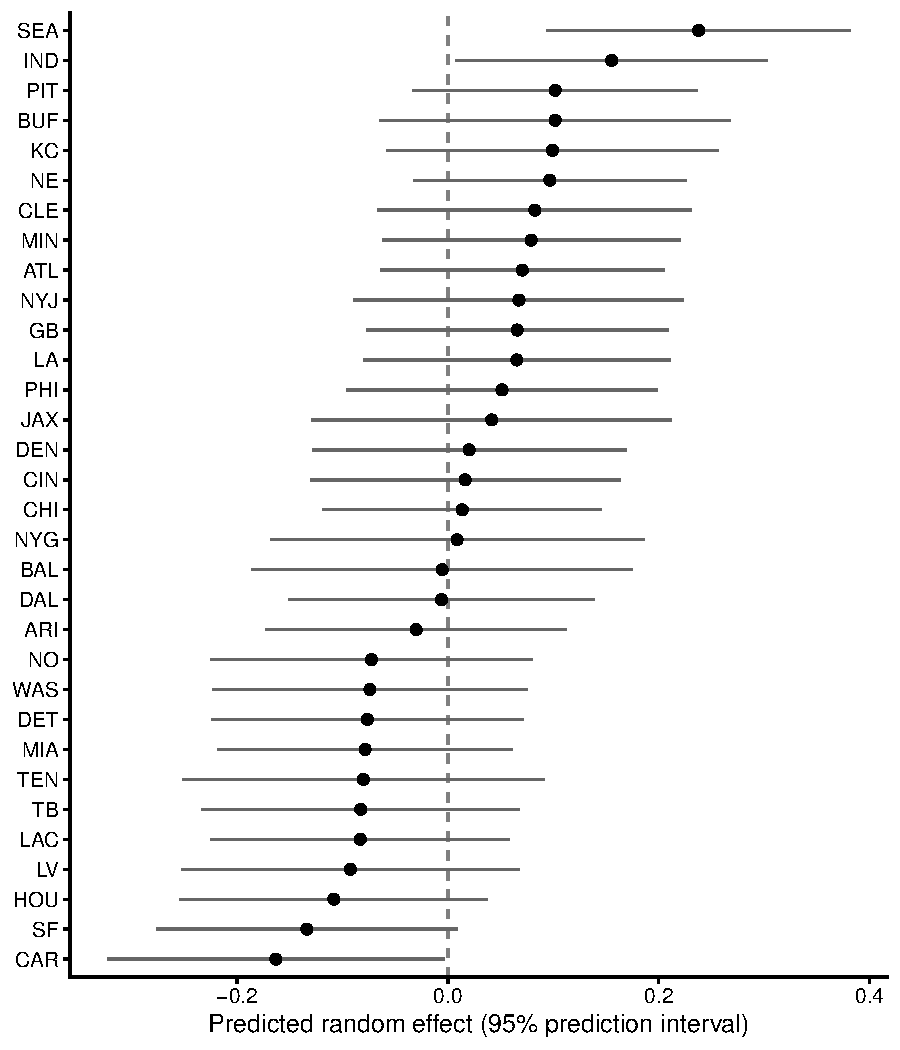
\includegraphics[width= \linewidth]{figures/plots/re_def.pdf}
    \caption{Predicted random effect for each defense. Smaller values correspond to a higher probability of staying in the respective state, i.e., continuing to cover a specific offensive player, and vice versa.}
    \label{fig:re_def}
\end{figure}
%\end{supplement}

\end{spacing}
\end{document}
